\documentclass[twoside]{book}

% Packages required by doxygen
\usepackage{fixltx2e}
\usepackage{calc}
\usepackage{doxygen}
\usepackage[export]{adjustbox} % also loads graphicx
\usepackage{graphicx}
\usepackage[utf8]{inputenc}
\usepackage{makeidx}
\usepackage{multicol}
\usepackage{multirow}
\PassOptionsToPackage{warn}{textcomp}
\usepackage{textcomp}
\usepackage[nointegrals]{wasysym}
\usepackage[table]{xcolor}

% Font selection
\usepackage[T1]{fontenc}
\usepackage[scaled=.90]{helvet}
\usepackage{courier}
\usepackage{amssymb}
\usepackage{sectsty}
\renewcommand{\familydefault}{\sfdefault}
\allsectionsfont{%
  \fontseries{bc}\selectfont%
  \color{darkgray}%
}
\renewcommand{\DoxyLabelFont}{%
  \fontseries{bc}\selectfont%
  \color{darkgray}%
}
\newcommand{\+}{\discretionary{\mbox{\scriptsize$\hookleftarrow$}}{}{}}

% Page & text layout
\usepackage{geometry}
\geometry{%
  a4paper,%
  top=2.5cm,%
  bottom=2.5cm,%
  left=2.5cm,%
  right=2.5cm%
}
\tolerance=750
\hfuzz=15pt
\hbadness=750
\setlength{\emergencystretch}{15pt}
\setlength{\parindent}{0cm}
\setlength{\parskip}{3ex plus 2ex minus 2ex}
\makeatletter
\renewcommand{\paragraph}{%
  \@startsection{paragraph}{4}{0ex}{-1.0ex}{1.0ex}{%
    \normalfont\normalsize\bfseries\SS@parafont%
  }%
}
\renewcommand{\subparagraph}{%
  \@startsection{subparagraph}{5}{0ex}{-1.0ex}{1.0ex}{%
    \normalfont\normalsize\bfseries\SS@subparafont%
  }%
}
\makeatother

% Headers & footers
\usepackage{fancyhdr}
\pagestyle{fancyplain}
\fancyhead[LE]{\fancyplain{}{\bfseries\thepage}}
\fancyhead[CE]{\fancyplain{}{}}
\fancyhead[RE]{\fancyplain{}{\bfseries\leftmark}}
\fancyhead[LO]{\fancyplain{}{\bfseries\rightmark}}
\fancyhead[CO]{\fancyplain{}{}}
\fancyhead[RO]{\fancyplain{}{\bfseries\thepage}}
\fancyfoot[LE]{\fancyplain{}{}}
\fancyfoot[CE]{\fancyplain{}{}}
\fancyfoot[RE]{\fancyplain{}{\bfseries\scriptsize Generated by Doxygen }}
\fancyfoot[LO]{\fancyplain{}{\bfseries\scriptsize Generated by Doxygen }}
\fancyfoot[CO]{\fancyplain{}{}}
\fancyfoot[RO]{\fancyplain{}{}}
\renewcommand{\footrulewidth}{0.4pt}
\renewcommand{\chaptermark}[1]{%
  \markboth{#1}{}%
}
\renewcommand{\sectionmark}[1]{%
  \markright{\thesection\ #1}%
}

% Indices & bibliography
\usepackage{natbib}
\usepackage[titles]{tocloft}
\setcounter{tocdepth}{3}
\setcounter{secnumdepth}{5}
\makeindex

% Hyperlinks (required, but should be loaded last)
\usepackage{ifpdf}
\ifpdf
  \usepackage[pdftex,pagebackref=true]{hyperref}
\else
  \usepackage[ps2pdf,pagebackref=true]{hyperref}
\fi
\hypersetup{%
  colorlinks=true,%
  linkcolor=blue,%
  citecolor=blue,%
  unicode%
}

% Custom commands
\newcommand{\clearemptydoublepage}{%
  \newpage{\pagestyle{empty}\cleardoublepage}%
}

\usepackage{caption}
\captionsetup{labelsep=space,justification=centering,font={bf},singlelinecheck=off,skip=4pt,position=top}

%===== C O N T E N T S =====

\begin{document}

% Titlepage & ToC
\hypersetup{pageanchor=false,
             bookmarksnumbered=true,
             pdfencoding=unicode
            }
\pagenumbering{alph}
\begin{titlepage}
\vspace*{7cm}
\begin{center}%
{\Large zpr\+\_\+projekt }\\
\vspace*{1cm}
{\large Generated by Doxygen 1.8.14}\\
\end{center}
\end{titlepage}
\clearemptydoublepage
\pagenumbering{roman}
\tableofcontents
\clearemptydoublepage
\pagenumbering{arabic}
\hypersetup{pageanchor=true}

%--- Begin generated contents ---
\chapter{Namespace Index}
\section{Namespace List}
Here is a list of all documented namespaces with brief descriptions\+:\begin{DoxyCompactList}
\item\contentsline{section}{\mbox{\hyperlink{namespace_ui}{Ui}} \\*Interfejs graficzny }{\pageref{namespace_ui}}{}
\end{DoxyCompactList}

\chapter{Hierarchical Index}
\section{Class Hierarchy}
This inheritance list is sorted roughly, but not completely, alphabetically\+:\begin{DoxyCompactList}
\item \contentsline{section}{Base}{\pageref{class_base}}{}
\begin{DoxyCompactList}
\item \contentsline{section}{Database}{\pageref{class_database}}{}
\item \contentsline{section}{Databases\+List}{\pageref{class_databases_list}}{}
\item \contentsline{section}{Element}{\pageref{class_element}}{}
\item \contentsline{section}{Picture}{\pageref{class_picture}}{}
\item \contentsline{section}{Word}{\pageref{class_word}}{}
\end{DoxyCompactList}
\item \contentsline{section}{Data\+Counter}{\pageref{class_data_counter}}{}
\item \contentsline{section}{Elements\+Database}{\pageref{class_elements_database}}{}
\begin{DoxyCompactList}
\item \contentsline{section}{Add\+Database\+Observer}{\pageref{class_add_database_observer}}{}
\item \contentsline{section}{Delete\+Database\+Observer}{\pageref{class_delete_database_observer}}{}
\end{DoxyCompactList}
\item Q\+Dialog\begin{DoxyCompactList}
\item \contentsline{section}{Delete\+Database\+Window}{\pageref{class_delete_database_window}}{}
\item \contentsline{section}{Dialog}{\pageref{class_dialog}}{}
\item \contentsline{section}{Get\+Database\+Name\+Window}{\pageref{class_get_database_name_window}}{}
\item \contentsline{section}{Menu\+Start}{\pageref{class_menu_start}}{}
\item \contentsline{section}{Message\+Window}{\pageref{class_message_window}}{}
\end{DoxyCompactList}
\item Q\+Main\+Window\begin{DoxyCompactList}
\item \contentsline{section}{Main\+Win}{\pageref{class_main_win}}{}
\end{DoxyCompactList}
\item Q\+Widget\begin{DoxyCompactList}
\item \contentsline{section}{Add\+Database\+Window}{\pageref{class_add_database_window}}{}
\item \contentsline{section}{Choose\+Database\+Window}{\pageref{class_choose_database_window}}{}
\end{DoxyCompactList}
\item \contentsline{section}{Repetition}{\pageref{class_repetition}}{}
\item \contentsline{section}{Ui\+\_\+\+Add\+Database\+Window}{\pageref{class_ui___add_database_window}}{}
\begin{DoxyCompactList}
\item \contentsline{section}{Ui\+:\+:Add\+Database\+Window}{\pageref{class_ui_1_1_add_database_window}}{}
\end{DoxyCompactList}
\item \contentsline{section}{Ui\+\_\+\+Choose\+Database\+Window}{\pageref{class_ui___choose_database_window}}{}
\begin{DoxyCompactList}
\item \contentsline{section}{Ui\+:\+:Choose\+Database\+Window}{\pageref{class_ui_1_1_choose_database_window}}{}
\end{DoxyCompactList}
\item \contentsline{section}{Ui\+\_\+\+Delete\+Database\+Window}{\pageref{class_ui___delete_database_window}}{}
\begin{DoxyCompactList}
\item \contentsline{section}{Ui\+:\+:Delete\+Database\+Window}{\pageref{class_ui_1_1_delete_database_window}}{}
\end{DoxyCompactList}
\item \contentsline{section}{Ui\+\_\+\+Get\+Database\+Name\+Window}{\pageref{class_ui___get_database_name_window}}{}
\begin{DoxyCompactList}
\item \contentsline{section}{Ui\+:\+:Get\+Database\+Name\+Window}{\pageref{class_ui_1_1_get_database_name_window}}{}
\end{DoxyCompactList}
\item \contentsline{section}{Ui\+\_\+\+Main\+Win}{\pageref{class_ui___main_win}}{}
\begin{DoxyCompactList}
\item \contentsline{section}{Ui\+:\+:Main\+Win}{\pageref{class_ui_1_1_main_win}}{}
\end{DoxyCompactList}
\item \contentsline{section}{Ui\+\_\+\+Menu\+Start}{\pageref{class_ui___menu_start}}{}
\begin{DoxyCompactList}
\item \contentsline{section}{Ui\+:\+:Menu\+Start}{\pageref{class_ui_1_1_menu_start}}{}
\end{DoxyCompactList}
\end{DoxyCompactList}

\chapter{Class Index}
\section{Class List}
Here are the classes, structs, unions and interfaces with brief descriptions\+:\begin{DoxyCompactList}
\item\contentsline{section}{\mbox{\hyperlink{class_add_database_observer}{Add\+Database\+Observer}} \\*Obserwator, w przypadku zmiany stanu dodaje nowy element do danej bazy danych }{\pageref{class_add_database_observer}}{}
\item\contentsline{section}{\mbox{\hyperlink{class_add_database_window}{Add\+Database\+Window}} \\*\mbox{\hyperlink{class_add_database_window}{Add\+Database\+Window}} okno które umożliwia użytkownikowi dodanie nowej bazy danych }{\pageref{class_add_database_window}}{}
\item\contentsline{section}{\mbox{\hyperlink{class_ui_1_1_add_database_window}{Ui\+::\+Add\+Database\+Window}} }{\pageref{class_ui_1_1_add_database_window}}{}
\item\contentsline{section}{\mbox{\hyperlink{class_base}{Base}} \\*Klasa bazowa dla klas, które dokonują operacji na plikach, dostarcza podstawe funkcje umożliwiające czytanie danych z pliku czy zapis danych }{\pageref{class_base}}{}
\item\contentsline{section}{\mbox{\hyperlink{class_choose_database_window}{Choose\+Database\+Window}} \\*Okno umożliwiające użytkownikowi wybór bazy danych do powtórki }{\pageref{class_choose_database_window}}{}
\item\contentsline{section}{\mbox{\hyperlink{class_ui_1_1_choose_database_window}{Ui\+::\+Choose\+Database\+Window}} }{\pageref{class_ui_1_1_choose_database_window}}{}
\item\contentsline{section}{\mbox{\hyperlink{class_database}{Database}} \\*Klasa \mbox{\hyperlink{class_database}{Database}} przechowuje informacje i parametry danej bazy danych }{\pageref{class_database}}{}
\item\contentsline{section}{\mbox{\hyperlink{class_databases_list}{Databases\+List}} \\*Klasa przechowująca liste dostępnych baz danych }{\pageref{class_databases_list}}{}
\item\contentsline{section}{\mbox{\hyperlink{class_data_counter}{Data\+Counter}} \\*Klasa pobiera aktualną datę oraz oblicza różnice pomiędzy tą daną a datą ostatniej powtórki danego elementu. Dzięki temu umożliwia określenie czy dany element powinnien znajdować się w liście do powtórzenia na dziś,czy nie }{\pageref{class_data_counter}}{}
\item\contentsline{section}{\mbox{\hyperlink{class_delete_database_observer}{Delete\+Database\+Observer}} \\*Umożliwia usunięcie danej bazy danych, informacje o tym która baza ma zostać usunięta pobiera od użytkownika }{\pageref{class_delete_database_observer}}{}
\item\contentsline{section}{\mbox{\hyperlink{class_delete_database_window}{Delete\+Database\+Window}} \\*Klasa reprezentująca okno, które umożliwia użykowinikowi wybór bazy danych do usunięcia. informajca o tym, która baza danych ma być usunięta jest przekazywana do odpowiedniego obserwatora }{\pageref{class_delete_database_window}}{}
\item\contentsline{section}{\mbox{\hyperlink{class_ui_1_1_delete_database_window}{Ui\+::\+Delete\+Database\+Window}} }{\pageref{class_ui_1_1_delete_database_window}}{}
\item\contentsline{section}{\mbox{\hyperlink{class_dialog}{Dialog}} }{\pageref{class_dialog}}{}
\item\contentsline{section}{\mbox{\hyperlink{class_element}{Element}} \\*Klasa reprezentująca pojedyńczy element z danej bazy, dostarcza funkcje umożliwiające zarządzanie danym elementem, w tym m.\+in zmianę jego stanu, zwiększenie lub zmniejszenie współczynnika zapamiętania itp }{\pageref{class_element}}{}
\item\contentsline{section}{\mbox{\hyperlink{class_elements_database}{Elements\+Database}} \\*Klasa reprezentuje daną bazę danych. Przechowuje informacje o bazie oraz jej elementy }{\pageref{class_elements_database}}{}
\item\contentsline{section}{\mbox{\hyperlink{class_ui_1_1_get_database_name_window}{Ui\+::\+Get\+Database\+Name\+Window}} }{\pageref{class_ui_1_1_get_database_name_window}}{}
\item\contentsline{section}{\mbox{\hyperlink{class_get_database_name_window}{Get\+Database\+Name\+Window}} \\*Klasa umożliwia użytkownikowi wpisanie nazwy nowododawanej bazy danych }{\pageref{class_get_database_name_window}}{}
\item\contentsline{section}{\mbox{\hyperlink{class_ui_1_1_main_win}{Ui\+::\+Main\+Win}} }{\pageref{class_ui_1_1_main_win}}{}
\item\contentsline{section}{\mbox{\hyperlink{class_main_win}{Main\+Win}} \\*Główne okno programu }{\pageref{class_main_win}}{}
\item\contentsline{section}{\mbox{\hyperlink{class_ui_1_1_menu_start}{Ui\+::\+Menu\+Start}} }{\pageref{class_ui_1_1_menu_start}}{}
\item\contentsline{section}{\mbox{\hyperlink{class_menu_start}{Menu\+Start}} \\*Klasam reprezentuje okno startowe, umożliwia użytkowi wybranie konkretnych akcji }{\pageref{class_menu_start}}{}
\item\contentsline{section}{\mbox{\hyperlink{class_picture}{Picture}} \\*Klasa przechowuje informacje o obrazku dołączonym do danego elementu }{\pageref{class_picture}}{}
\item\contentsline{section}{\mbox{\hyperlink{class_repetition}{Repetition}} \\*Klasa reprezentuje aktualna powtórkę, przechowuje tylko te elementy danej bazy które należy powtórzyć w danym dniu. Umożliwia kolejne wyświetlanie elementów w głownym oknie programu }{\pageref{class_repetition}}{}
\item\contentsline{section}{\mbox{\hyperlink{class_ui___add_database_window}{Ui\+\_\+\+Add\+Database\+Window}} }{\pageref{class_ui___add_database_window}}{}
\item\contentsline{section}{\mbox{\hyperlink{class_ui___choose_database_window}{Ui\+\_\+\+Choose\+Database\+Window}} }{\pageref{class_ui___choose_database_window}}{}
\item\contentsline{section}{\mbox{\hyperlink{class_ui___delete_database_window}{Ui\+\_\+\+Delete\+Database\+Window}} }{\pageref{class_ui___delete_database_window}}{}
\item\contentsline{section}{\mbox{\hyperlink{class_ui___get_database_name_window}{Ui\+\_\+\+Get\+Database\+Name\+Window}} }{\pageref{class_ui___get_database_name_window}}{}
\item\contentsline{section}{\mbox{\hyperlink{class_ui___main_win}{Ui\+\_\+\+Main\+Win}} }{\pageref{class_ui___main_win}}{}
\item\contentsline{section}{\mbox{\hyperlink{class_ui___menu_start}{Ui\+\_\+\+Menu\+Start}} }{\pageref{class_ui___menu_start}}{}
\item\contentsline{section}{\mbox{\hyperlink{class_word}{Word}} \\*Klasa reprezentuje dane słówko, które może być zapisane w dwóch językach oraz posiadac pewien synonim lub opis. dostarcza funkcji umożliwających modyfikacje słówka oraz jego zapis i odczyt z /do pliku }{\pageref{class_word}}{}
\end{DoxyCompactList}

\chapter{Namespace Documentation}
\hypertarget{namespace_ui}{}\section{Ui Namespace Reference}
\label{namespace_ui}\index{Ui@{Ui}}


interfejs graficzny  


\subsection*{Classes}
\begin{DoxyCompactItemize}
\item 
class \mbox{\hyperlink{class_ui_1_1_add_database_window}{Add\+Database\+Window}}
\item 
class \mbox{\hyperlink{class_ui_1_1_choose_database_window}{Choose\+Database\+Window}}
\item 
class \mbox{\hyperlink{class_ui_1_1_delete_database_window}{Delete\+Database\+Window}}
\item 
class \mbox{\hyperlink{class_ui_1_1_get_database_name_window}{Get\+Database\+Name\+Window}}
\item 
class \mbox{\hyperlink{class_ui_1_1_main_win}{Main\+Win}}
\item 
class \mbox{\hyperlink{class_ui_1_1_menu_start}{Menu\+Start}}
\end{DoxyCompactItemize}


\subsection{Detailed Description}
interfejs graficzny 
\chapter{Class Documentation}
\hypertarget{class_add_database_observer}{}\section{Add\+Database\+Observer Class Reference}
\label{class_add_database_observer}\index{Add\+Database\+Observer@{Add\+Database\+Observer}}


Obserwator, w przypadku zmiany stanu dodaje nowy element do danej bazy danych.  




{\ttfamily \#include $<$adddatabaseobserver.\+h$>$}

Inheritance diagram for Add\+Database\+Observer\+:\begin{figure}[H]
\begin{center}
\leavevmode
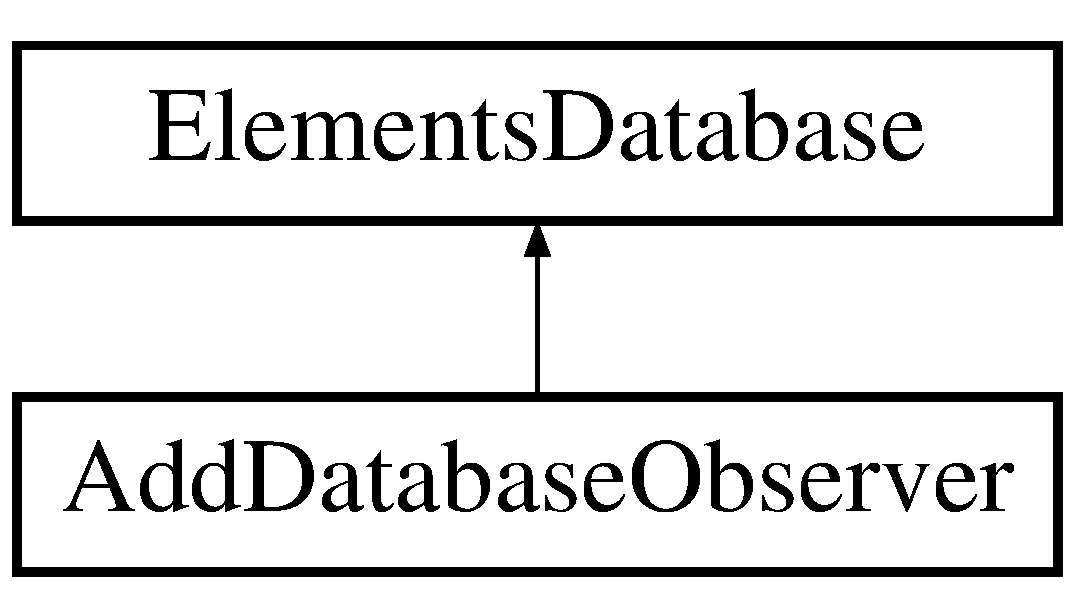
\includegraphics[height=2.000000cm]{class_add_database_observer}
\end{center}
\end{figure}
\subsection*{Public Member Functions}
\begin{DoxyCompactItemize}
\item 
virtual void \mbox{\hyperlink{class_add_database_observer_a6f2bc1af6f2887b326c40d2efec9cf42}{update}} (\mbox{\hyperlink{class_element}{Element}} new\+\_\+element)
\begin{DoxyCompactList}\small\item\em update -\/ funkja umozliwiająca dodanie nowego elementu do danej bazy danych \end{DoxyCompactList}\end{DoxyCompactItemize}
\subsection*{Additional Inherited Members}


\subsection{Detailed Description}
Obserwator, w przypadku zmiany stanu dodaje nowy element do danej bazy danych. 

\subsection{Member Function Documentation}
\mbox{\Hypertarget{class_add_database_observer_a6f2bc1af6f2887b326c40d2efec9cf42}\label{class_add_database_observer_a6f2bc1af6f2887b326c40d2efec9cf42}} 
\index{Add\+Database\+Observer@{Add\+Database\+Observer}!update@{update}}
\index{update@{update}!Add\+Database\+Observer@{Add\+Database\+Observer}}
\subsubsection{\texorpdfstring{update()}{update()}}
{\footnotesize\ttfamily void Add\+Database\+Observer\+::update (\begin{DoxyParamCaption}\item[{\mbox{\hyperlink{class_element}{Element}}}]{new\+\_\+element }\end{DoxyParamCaption})\hspace{0.3cm}{\ttfamily [virtual]}}



update -\/ funkja umozliwiająca dodanie nowego elementu do danej bazy danych 


\begin{DoxyParams}{Parameters}
{\em new\+\_\+element} & -\/ nowy element, ktory ma zostac dodany \\
\hline
\end{DoxyParams}


The documentation for this class was generated from the following files\+:\begin{DoxyCompactItemize}
\item 
adddatabaseobserver.\+h\item 
adddatabaseobserver.\+cpp\end{DoxyCompactItemize}

\hypertarget{class_add_database_window}{}\section{Add\+Database\+Window Class Reference}
\label{class_add_database_window}\index{Add\+Database\+Window@{Add\+Database\+Window}}


\mbox{\hyperlink{class_add_database_window}{Add\+Database\+Window}} okno które umożliwia użytkownikowi dodanie nowej bazy danych.  




{\ttfamily \#include $<$adddatabasewindow.\+h$>$}

Inheritance diagram for Add\+Database\+Window\+:\begin{figure}[H]
\begin{center}
\leavevmode
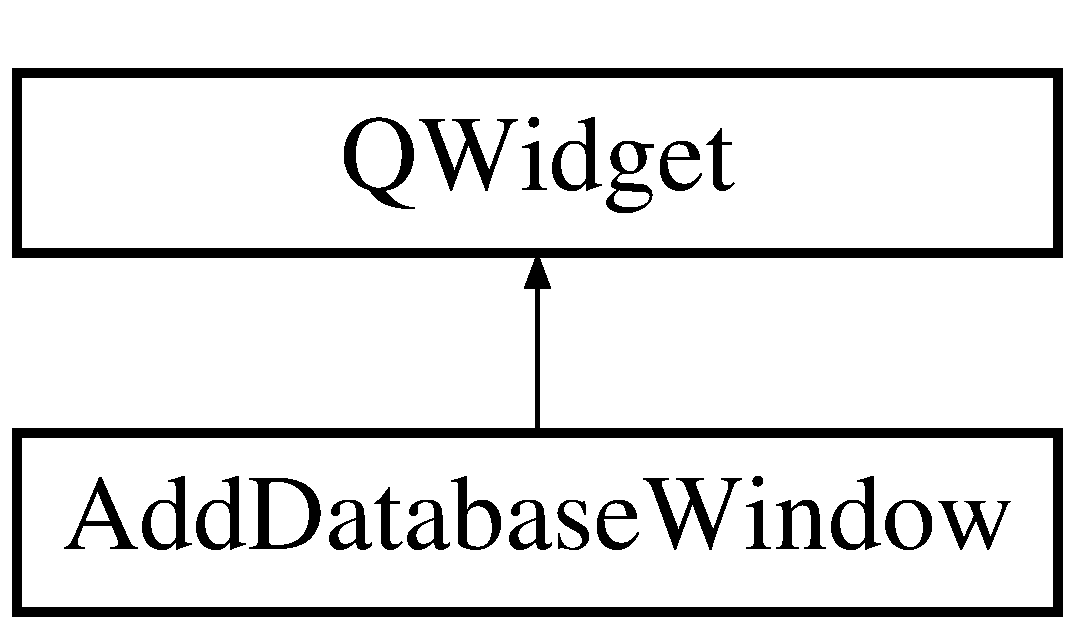
\includegraphics[height=2.000000cm]{class_add_database_window}
\end{center}
\end{figure}
\subsection*{Public Member Functions}
\begin{DoxyCompactItemize}
\item 
\mbox{\Hypertarget{class_add_database_window_aaab147e23b2461e5282bbc6dac3594a5}\label{class_add_database_window_aaab147e23b2461e5282bbc6dac3594a5}} 
{\bfseries Add\+Database\+Window} (Q\+Widget $\ast$parent=0, \mbox{\hyperlink{class_menu_start}{Menu\+Start}} $\ast$menu=0)
\item 
\mbox{\Hypertarget{class_add_database_window_a894d5c23c4772452781872f9393dc2b4}\label{class_add_database_window_a894d5c23c4772452781872f9393dc2b4}} 
void {\bfseries notify} ()
\item 
\mbox{\Hypertarget{class_add_database_window_a95c48c7ed785580c33f707f75ee132ad}\label{class_add_database_window_a95c48c7ed785580c33f707f75ee132ad}} 
void {\bfseries write\+To\+File} (std\+::string file\+\_\+name)
\item 
\mbox{\Hypertarget{class_add_database_window_aba798c1e673e4194434ceffa62cda4fa}\label{class_add_database_window_aba798c1e673e4194434ceffa62cda4fa}} 
bool {\bfseries set\+Database\+Name} (std\+::string new\+\_\+name)
\end{DoxyCompactItemize}


\subsection{Detailed Description}
\mbox{\hyperlink{class_add_database_window}{Add\+Database\+Window}} okno które umożliwia użytkownikowi dodanie nowej bazy danych. 

The documentation for this class was generated from the following files\+:\begin{DoxyCompactItemize}
\item 
adddatabasewindow.\+h\item 
adddatabasewindow.\+cpp\end{DoxyCompactItemize}

\hypertarget{class_ui_1_1_add_database_window}{}\section{Ui\+:\+:Add\+Database\+Window Class Reference}
\label{class_ui_1_1_add_database_window}\index{Ui\+::\+Add\+Database\+Window@{Ui\+::\+Add\+Database\+Window}}
Inheritance diagram for Ui\+:\+:Add\+Database\+Window\+:\begin{figure}[H]
\begin{center}
\leavevmode
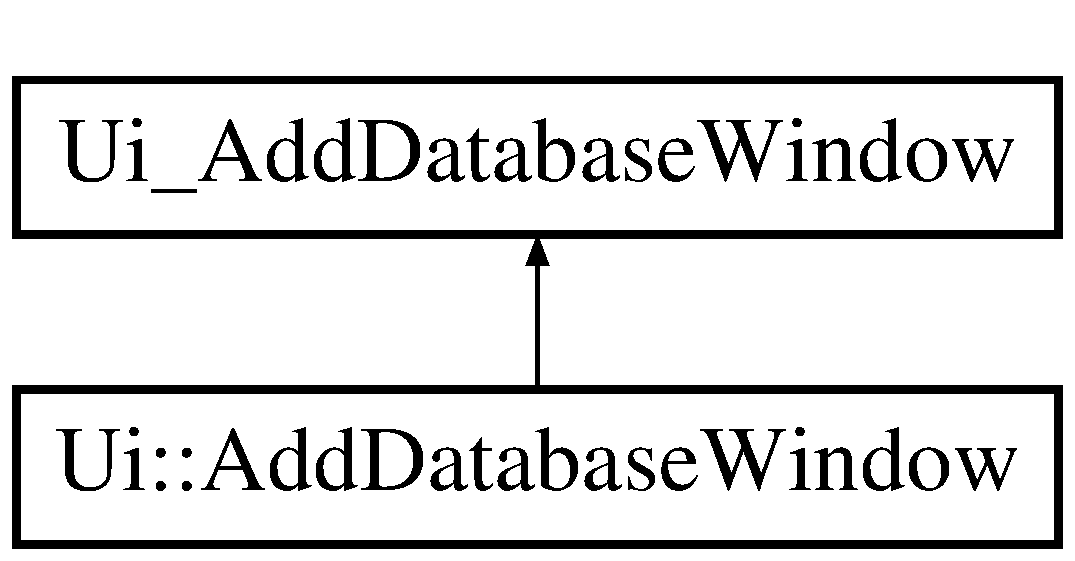
\includegraphics[height=2.000000cm]{class_ui_1_1_add_database_window}
\end{center}
\end{figure}
\subsection*{Additional Inherited Members}


The documentation for this class was generated from the following file\+:\begin{DoxyCompactItemize}
\item 
ui\+\_\+adddatabasewindow.\+h\end{DoxyCompactItemize}

\hypertarget{class_base}{}\section{Base Class Reference}
\label{class_base}\index{Base@{Base}}


\mbox{\hyperlink{class_base}{Base}} jest klasą bazową dla klas, które dokonują operacji na plikach, dostarcza podstawe funkcje umożliwiające czytanie danych z pliku czy zapis danych.  




{\ttfamily \#include $<$base.\+h$>$}

Inheritance diagram for Base\+:\begin{figure}[H]
\begin{center}
\leavevmode
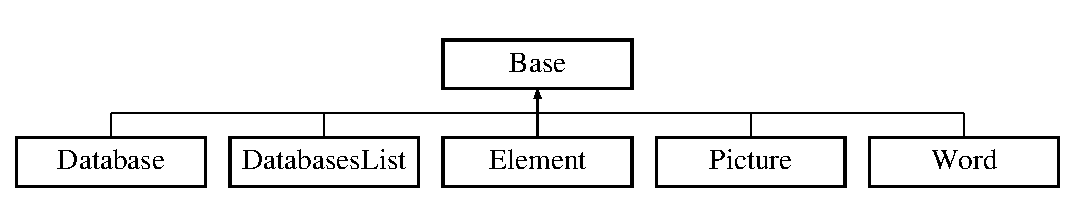
\includegraphics[height=2.000000cm]{class_base}
\end{center}
\end{figure}
\subsection*{Public Member Functions}
\begin{DoxyCompactItemize}
\item 
\mbox{\Hypertarget{class_base_a7b4b21d52b3d3247744e0ee1e4f63586}\label{class_base_a7b4b21d52b3d3247744e0ee1e4f63586}} 
virtual void {\bfseries import\+Data} (std\+::istream \&in\+\_\+)=0
\item 
\mbox{\Hypertarget{class_base_a88840038845318752f245aeec2ea4a68}\label{class_base_a88840038845318752f245aeec2ea4a68}} 
virtual void {\bfseries export\+Data} (std\+::ostream \&out\+\_\+)=0
\item 
\mbox{\Hypertarget{class_base_ac414e12b727e044fd3a56ca6d8c1d4e6}\label{class_base_ac414e12b727e044fd3a56ca6d8c1d4e6}} 
virtual void {\bfseries read\+From\+File} (std\+::string file\+\_\+name)
\item 
\mbox{\Hypertarget{class_base_ae878e796ec7e77f33ebee2048f961551}\label{class_base_ae878e796ec7e77f33ebee2048f961551}} 
virtual void {\bfseries write\+To\+File} (std\+::string file\+\_\+name)
\item 
\mbox{\Hypertarget{class_base_a4d31c87adaa91feaecf96d09825caacc}\label{class_base_a4d31c87adaa91feaecf96d09825caacc}} 
virtual void {\bfseries set\+Name} (std\+::string name)
\item 
\mbox{\Hypertarget{class_base_abc24d7d976d415e2facc4e2d2cc0730d}\label{class_base_abc24d7d976d415e2facc4e2d2cc0730d}} 
virtual std\+::string {\bfseries get\+Name} ()
\end{DoxyCompactItemize}
\subsection*{Protected Attributes}
\begin{DoxyCompactItemize}
\item 
\mbox{\Hypertarget{class_base_ace990b7abe15279f1bcf958f3a1f0d6b}\label{class_base_ace990b7abe15279f1bcf958f3a1f0d6b}} 
std\+::string {\bfseries name\+\_\+} =\char`\"{}none\char`\"{}
\end{DoxyCompactItemize}


\subsection{Detailed Description}
\mbox{\hyperlink{class_base}{Base}} jest klasą bazową dla klas, które dokonują operacji na plikach, dostarcza podstawe funkcje umożliwiające czytanie danych z pliku czy zapis danych. 

The documentation for this class was generated from the following files\+:\begin{DoxyCompactItemize}
\item 
base.\+h\item 
base.\+cpp\end{DoxyCompactItemize}

\hypertarget{class_choose_database_window}{}\section{Choose\+Database\+Window Class Reference}
\label{class_choose_database_window}\index{Choose\+Database\+Window@{Choose\+Database\+Window}}


okno umożliwiające użytkownikowi wybór bazy danych do powtórki  




{\ttfamily \#include $<$choosedatabasewindow.\+h$>$}

Inheritance diagram for Choose\+Database\+Window\+:\begin{figure}[H]
\begin{center}
\leavevmode
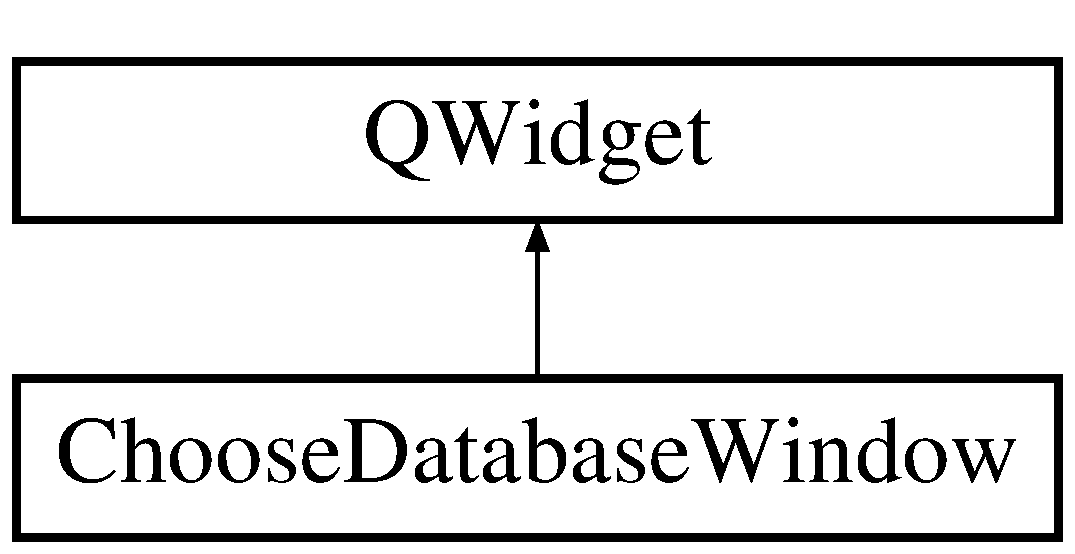
\includegraphics[height=2.000000cm]{class_choose_database_window}
\end{center}
\end{figure}
\subsection*{Public Member Functions}
\begin{DoxyCompactItemize}
\item 
\mbox{\Hypertarget{class_choose_database_window_a97a5d367fea9c9f51cf74e898626c5a8}\label{class_choose_database_window_a97a5d367fea9c9f51cf74e898626c5a8}} 
{\bfseries Choose\+Database\+Window} (Q\+Widget $\ast$parent=0, \mbox{\hyperlink{class_menu_start}{Menu\+Start}} $\ast$menu\+\_\+start\+\_\+=0, \mbox{\hyperlink{class_main_win}{Main\+Win}} $\ast$main\+\_\+window\+\_\+=0)
\item 
\mbox{\Hypertarget{class_choose_database_window_a8bb827c6d1f1e60a1ea091c8ff9ef591}\label{class_choose_database_window_a8bb827c6d1f1e60a1ea091c8ff9ef591}} 
void {\bfseries show\+Databases\+List} ()
\item 
\mbox{\Hypertarget{class_choose_database_window_aa63c9e154637a45f33da4354a4761bce}\label{class_choose_database_window_aa63c9e154637a45f33da4354a4761bce}} 
int {\bfseries show\+Message\+Window} (Q\+String info\+\_\+text)
\end{DoxyCompactItemize}


\subsection{Detailed Description}
okno umożliwiające użytkownikowi wybór bazy danych do powtórki 

The documentation for this class was generated from the following files\+:\begin{DoxyCompactItemize}
\item 
choosedatabasewindow.\+h\item 
choosedatabasewindow.\+cpp\end{DoxyCompactItemize}

\hypertarget{class_ui_1_1_choose_database_window}{}\section{Ui\+:\+:Choose\+Database\+Window Class Reference}
\label{class_ui_1_1_choose_database_window}\index{Ui\+::\+Choose\+Database\+Window@{Ui\+::\+Choose\+Database\+Window}}
Inheritance diagram for Ui\+:\+:Choose\+Database\+Window\+:\begin{figure}[H]
\begin{center}
\leavevmode
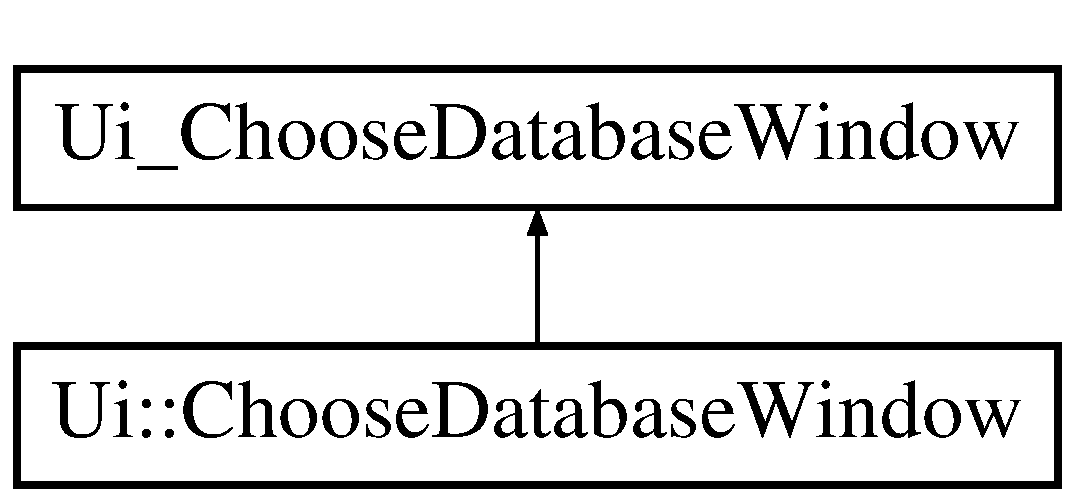
\includegraphics[height=2.000000cm]{class_ui_1_1_choose_database_window}
\end{center}
\end{figure}
\subsection*{Additional Inherited Members}


The documentation for this class was generated from the following file\+:\begin{DoxyCompactItemize}
\item 
ui\+\_\+choosedatabasewindow.\+h\end{DoxyCompactItemize}

\hypertarget{class_database}{}\section{Database Class Reference}
\label{class_database}\index{Database@{Database}}


Klasa \mbox{\hyperlink{class_database}{Database}} przechowuje informacje i parametry danej bazy danych.  




{\ttfamily \#include $<$database.\+h$>$}

Inheritance diagram for Database\+:\begin{figure}[H]
\begin{center}
\leavevmode
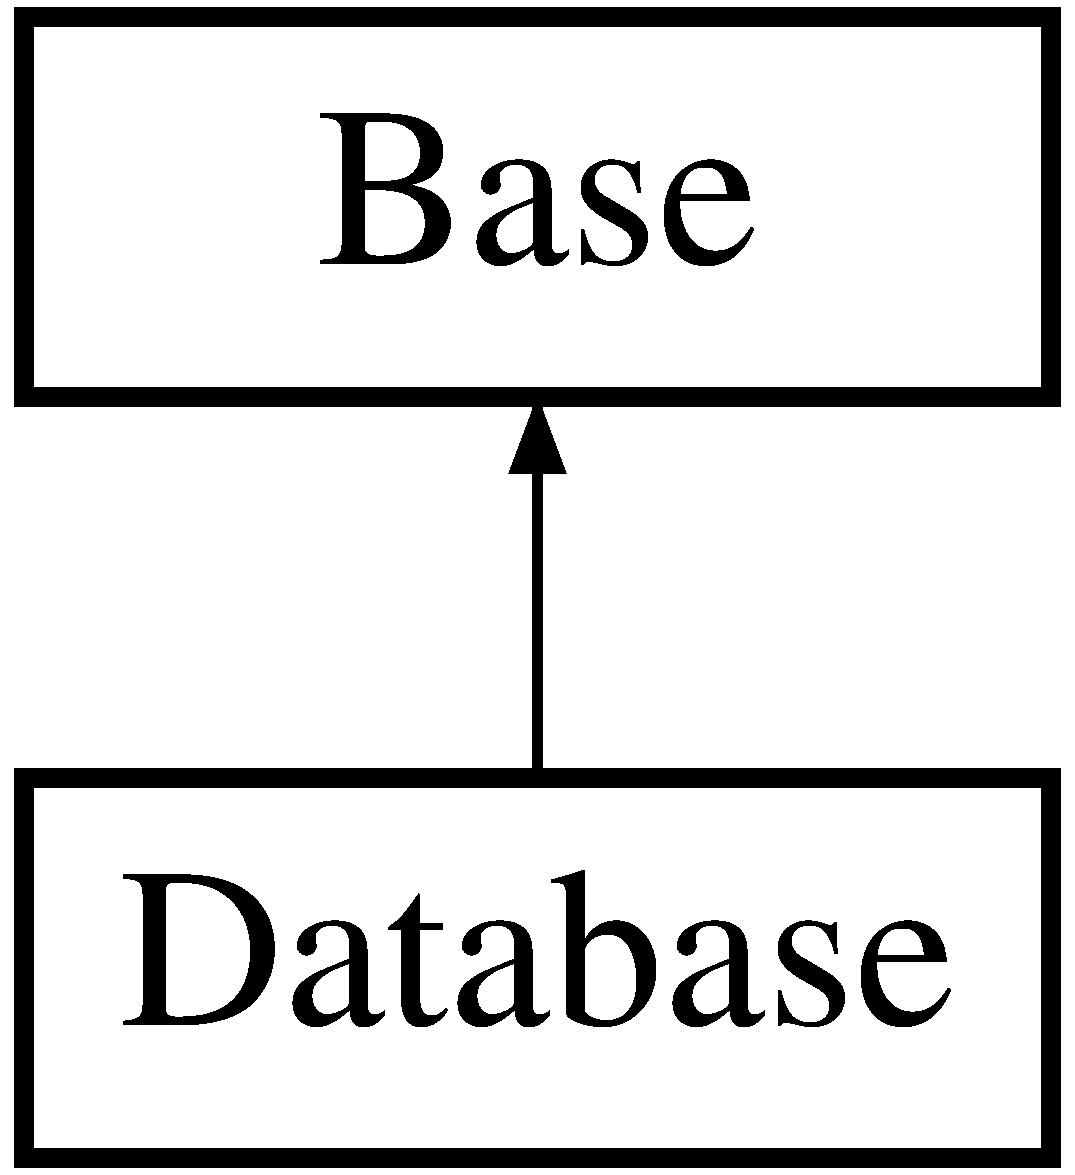
\includegraphics[height=2.000000cm]{class_database}
\end{center}
\end{figure}
\subsection*{Public Member Functions}
\begin{DoxyCompactItemize}
\item 
\mbox{\Hypertarget{class_database_ad2ed7fa7af20809f84b7b13cd55ac9ef}\label{class_database_ad2ed7fa7af20809f84b7b13cd55ac9ef}} 
{\bfseries Database} (std\+::string name=\char`\"{} \char`\"{})
\item 
\mbox{\Hypertarget{class_database_aab7af7898890481802ae8c62b745bbe9}\label{class_database_aab7af7898890481802ae8c62b745bbe9}} 
virtual void {\bfseries import\+Data} (std\+::istream \&in\+\_\+)
\item 
\mbox{\Hypertarget{class_database_a79ff4cee1ef72bb7be0077c3553bd1e9}\label{class_database_a79ff4cee1ef72bb7be0077c3553bd1e9}} 
virtual void {\bfseries export\+Data} (std\+::ostream \&out\+\_\+)
\item 
\mbox{\Hypertarget{class_database_a68de399557003ffde43f6556237ee7f2}\label{class_database_a68de399557003ffde43f6556237ee7f2}} 
virtual void {\bfseries add} (\mbox{\hyperlink{class_base}{Base}} $\ast$)
\item 
\mbox{\Hypertarget{class_database_af757aa5b00ad981c6d3d2c9100694b0d}\label{class_database_af757aa5b00ad981c6d3d2c9100694b0d}} 
std\+::string {\bfseries get\+File\+Name} ()
\item 
\mbox{\Hypertarget{class_database_a84fe6d325d05ff32c513fd2763d69e57}\label{class_database_a84fe6d325d05ff32c513fd2763d69e57}} 
void {\bfseries set\+File\+Name} (std\+::string file\+\_\+name)
\item 
\mbox{\Hypertarget{class_database_a60f291231bd1bf8e7bc40a06d44b5d81}\label{class_database_a60f291231bd1bf8e7bc40a06d44b5d81}} 
void {\bfseries set\+Default\+File\+Name} ()
\item 
\mbox{\Hypertarget{class_database_ade24eccecba190ccd540b2bb2527d2d5}\label{class_database_ade24eccecba190ccd540b2bb2527d2d5}} 
std\+::string {\bfseries get\+Databases\+File\+Name} ()
\item 
\mbox{\Hypertarget{class_database_aea49c371662e5a5c80c5af44314fd7e8}\label{class_database_aea49c371662e5a5c80c5af44314fd7e8}} 
void {\bfseries increase\+Elements\+Number} ()
\item 
\mbox{\Hypertarget{class_database_aae945bd22e9b28da21cba4483d7d38ba}\label{class_database_aae945bd22e9b28da21cba4483d7d38ba}} 
unsigned int {\bfseries get\+Elements\+Number} ()
\item 
\mbox{\Hypertarget{class_database_a254f1f7b0721de43ea3e203009741305}\label{class_database_a254f1f7b0721de43ea3e203009741305}} 
bool {\bfseries delete\+Database} ()
\end{DoxyCompactItemize}
\subsection*{Additional Inherited Members}


\subsection{Detailed Description}
Klasa \mbox{\hyperlink{class_database}{Database}} przechowuje informacje i parametry danej bazy danych. 

The documentation for this class was generated from the following files\+:\begin{DoxyCompactItemize}
\item 
database.\+h\item 
database.\+cpp\end{DoxyCompactItemize}

\hypertarget{class_databases_list}{}\section{Databases\+List Class Reference}
\label{class_databases_list}\index{Databases\+List@{Databases\+List}}


Klasa przechowująca liste dostępnych baz danych.  




{\ttfamily \#include $<$databaseslist.\+h$>$}

Inheritance diagram for Databases\+List\+:\begin{figure}[H]
\begin{center}
\leavevmode
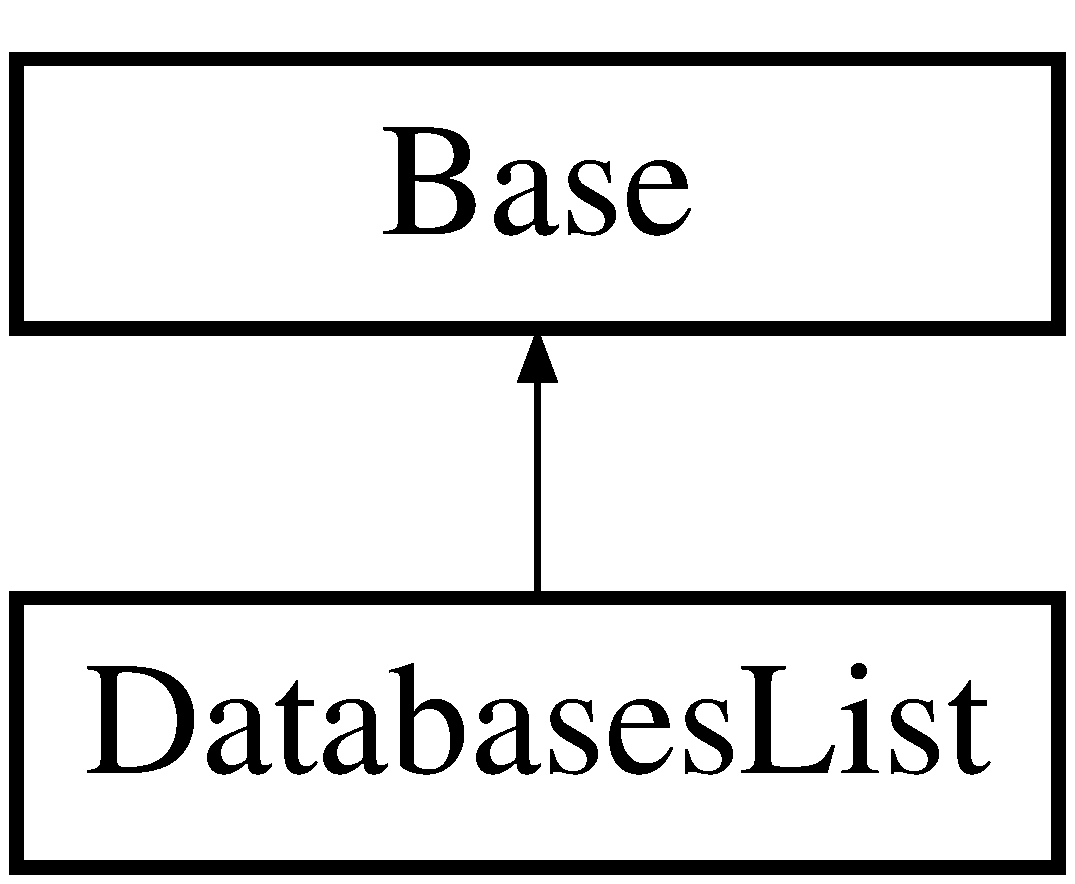
\includegraphics[height=2.000000cm]{class_databases_list}
\end{center}
\end{figure}
\subsection*{Public Member Functions}
\begin{DoxyCompactItemize}
\item 
\mbox{\Hypertarget{class_databases_list_abd187b9e0cf5551d63bcd76d97cd792e}\label{class_databases_list_abd187b9e0cf5551d63bcd76d97cd792e}} 
virtual void {\bfseries import\+Data} (std\+::istream \&in\+\_\+)
\item 
\mbox{\Hypertarget{class_databases_list_a0dc8aa3a016c4f466a3625f897d4b79a}\label{class_databases_list_a0dc8aa3a016c4f466a3625f897d4b79a}} 
virtual void {\bfseries export\+Data} (std\+::ostream \&out\+\_\+)
\item 
\mbox{\Hypertarget{class_databases_list_ada9be7bc8acb9bfe0ca59b3dc515afa7}\label{class_databases_list_ada9be7bc8acb9bfe0ca59b3dc515afa7}} 
virtual void {\bfseries read\+From\+File} ()
\item 
\mbox{\Hypertarget{class_databases_list_a2e64d5ee70b19c3056a63823c0191070}\label{class_databases_list_a2e64d5ee70b19c3056a63823c0191070}} 
virtual void {\bfseries write\+To\+File} ()
\item 
\mbox{\Hypertarget{class_databases_list_a36e4a59130a119f44e3ae18870d1a691}\label{class_databases_list_a36e4a59130a119f44e3ae18870d1a691}} 
virtual void {\bfseries add} (\mbox{\hyperlink{class_base}{Base}} $\ast$)
\item 
\mbox{\Hypertarget{class_databases_list_a97a1a3e49fb1644ab07999dc332a0efa}\label{class_databases_list_a97a1a3e49fb1644ab07999dc332a0efa}} 
virtual void {\bfseries add} (\mbox{\hyperlink{class_database}{Database}} new\+\_\+database)
\item 
\mbox{\Hypertarget{class_databases_list_a86f5b675c610750ba64ae1f494df687f}\label{class_databases_list_a86f5b675c610750ba64ae1f494df687f}} 
virtual unsigned int {\bfseries get\+Databases\+Number} ()
\item 
\mbox{\Hypertarget{class_databases_list_a054378c1becba066855c2daee11fbec7}\label{class_databases_list_a054378c1becba066855c2daee11fbec7}} 
std\+::vector$<$ std\+::string $>$ {\bfseries get\+Databases\+Names} ()
\item 
\mbox{\Hypertarget{class_databases_list_afcbaa3e3e622bd99276dfce327469e07}\label{class_databases_list_afcbaa3e3e622bd99276dfce327469e07}} 
\mbox{\hyperlink{class_database}{Database}} $\ast$ {\bfseries find\+Database} (std\+::string database\+\_\+name)
\item 
\mbox{\Hypertarget{class_databases_list_a48895e73772682d7a18ca170ff520068}\label{class_databases_list_a48895e73772682d7a18ca170ff520068}} 
void {\bfseries erase\+Database} (std\+::string database\+\_\+name)
\end{DoxyCompactItemize}
\subsection*{Static Public Member Functions}
\begin{DoxyCompactItemize}
\item 
\mbox{\Hypertarget{class_databases_list_a2e1bc9475b1b28106fe2d0b32fb0db1a}\label{class_databases_list_a2e1bc9475b1b28106fe2d0b32fb0db1a}} 
static \mbox{\hyperlink{class_databases_list}{Databases\+List}} $\ast$ {\bfseries get\+Instance} ()
\end{DoxyCompactItemize}
\subsection*{Additional Inherited Members}


\subsection{Detailed Description}
Klasa przechowująca liste dostępnych baz danych. 

The documentation for this class was generated from the following files\+:\begin{DoxyCompactItemize}
\item 
databaseslist.\+h\item 
databaseslist.\+cpp\end{DoxyCompactItemize}

\hypertarget{class_data_counter}{}\section{Data\+Counter Class Reference}
\label{class_data_counter}\index{Data\+Counter@{Data\+Counter}}


Klasa \mbox{\hyperlink{class_data_counter}{Data\+Counter}} pobiera aktualną datę oraz oblicza różnice pomiędzy tą daną a datą ostatniej powtórki danego elementu. Dzięki temu umożliwia określenie czy dany element powinnien znajdować się w liście do powtórzenia na dziś,czy nie.  




{\ttfamily \#include $<$datacounter.\+h$>$}

\subsection*{Public Member Functions}
\begin{DoxyCompactItemize}
\item 
\mbox{\Hypertarget{class_data_counter_ad3b3cb7addf5e0dbb8d5a76220884717}\label{class_data_counter_ad3b3cb7addf5e0dbb8d5a76220884717}} 
void {\bfseries set\+Current\+Data} ()
\item 
\mbox{\Hypertarget{class_data_counter_adf801ff96f2fa290fa0d65ccfabd5d84}\label{class_data_counter_adf801ff96f2fa290fa0d65ccfabd5d84}} 
int {\bfseries get\+Days\+Difference} (struct std\+::tm data\+\_\+)
\item 
\mbox{\Hypertarget{class_data_counter_a698e215d52c6b1634397273877a14a24}\label{class_data_counter_a698e215d52c6b1634397273877a14a24}} 
struct std\+::tm {\bfseries get\+Current\+Data} ()
\end{DoxyCompactItemize}
\subsection*{Static Public Member Functions}
\begin{DoxyCompactItemize}
\item 
\mbox{\Hypertarget{class_data_counter_a92a2b021515881d1ed48249a88f4e1cf}\label{class_data_counter_a92a2b021515881d1ed48249a88f4e1cf}} 
static \mbox{\hyperlink{class_data_counter}{Data\+Counter}} $\ast$ {\bfseries get\+Instance} ()
\end{DoxyCompactItemize}


\subsection{Detailed Description}
Klasa \mbox{\hyperlink{class_data_counter}{Data\+Counter}} pobiera aktualną datę oraz oblicza różnice pomiędzy tą daną a datą ostatniej powtórki danego elementu. Dzięki temu umożliwia określenie czy dany element powinnien znajdować się w liście do powtórzenia na dziś,czy nie. 

The documentation for this class was generated from the following files\+:\begin{DoxyCompactItemize}
\item 
datacounter.\+h\item 
datacounter.\+cpp\end{DoxyCompactItemize}

\hypertarget{class_delete_database_observer}{}\section{Delete\+Database\+Observer Class Reference}
\label{class_delete_database_observer}\index{Delete\+Database\+Observer@{Delete\+Database\+Observer}}


Umożliwia usunięcie danej bazy danych, informacje o tym która baza ma zostać usunięta pobiera od użytkownika.  




{\ttfamily \#include $<$deletedatabaseobserver.\+h$>$}

Inheritance diagram for Delete\+Database\+Observer\+:\begin{figure}[H]
\begin{center}
\leavevmode
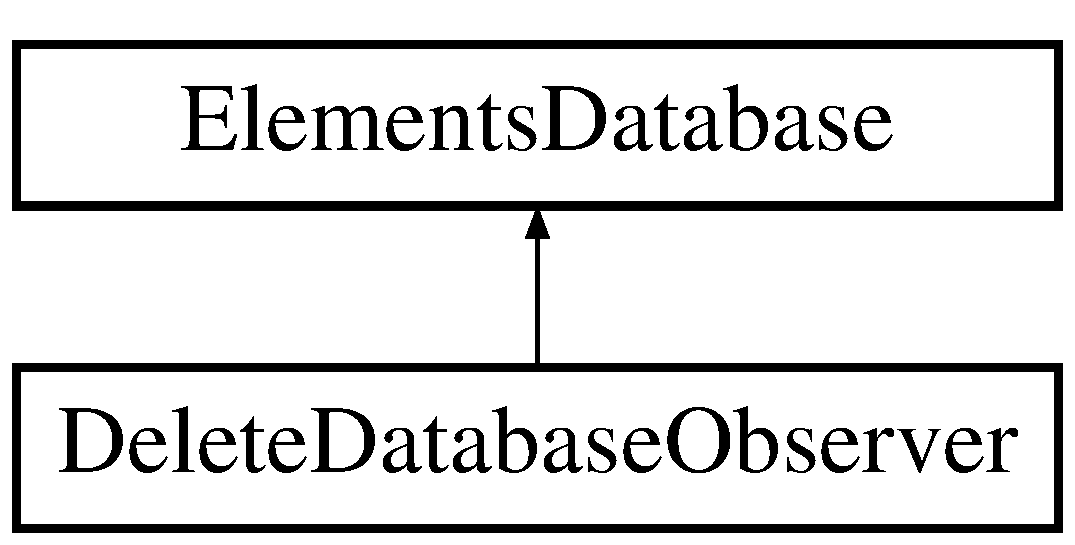
\includegraphics[height=2.000000cm]{class_delete_database_observer}
\end{center}
\end{figure}
\subsection*{Public Member Functions}
\begin{DoxyCompactItemize}
\item 
\mbox{\Hypertarget{class_delete_database_observer_aac4b2fa8fd6c4d160fd39e2d3fb0d1a0}\label{class_delete_database_observer_aac4b2fa8fd6c4d160fd39e2d3fb0d1a0}} 
virtual void {\bfseries update} (std\+::string database\+\_\+name)
\end{DoxyCompactItemize}
\subsection*{Additional Inherited Members}


\subsection{Detailed Description}
Umożliwia usunięcie danej bazy danych, informacje o tym która baza ma zostać usunięta pobiera od użytkownika. 

The documentation for this class was generated from the following files\+:\begin{DoxyCompactItemize}
\item 
deletedatabaseobserver.\+h\item 
deletedatabaseobserver.\+cpp\end{DoxyCompactItemize}

\hypertarget{class_delete_database_window}{}\section{Delete\+Database\+Window Class Reference}
\label{class_delete_database_window}\index{Delete\+Database\+Window@{Delete\+Database\+Window}}


Klasa reprezentująca okno, które umożliwia użykowinikowi wybór bazy danych do usunięcia. informajca o tym, która baza danych ma być usunięta jest przekazywana do odpowiedniego obserwatora.  




{\ttfamily \#include $<$deletedatabasewindow.\+h$>$}

Inheritance diagram for Delete\+Database\+Window\+:\begin{figure}[H]
\begin{center}
\leavevmode
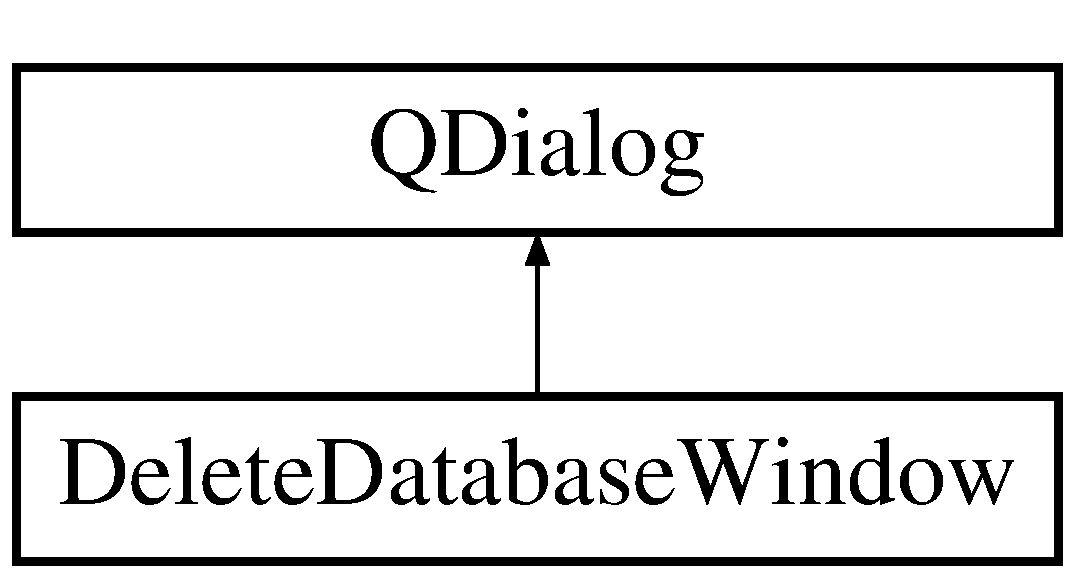
\includegraphics[height=2.000000cm]{class_delete_database_window}
\end{center}
\end{figure}
\subsection*{Public Member Functions}
\begin{DoxyCompactItemize}
\item 
\mbox{\Hypertarget{class_delete_database_window_ad7444fa62ecdc1353ba6a732b2032c9f}\label{class_delete_database_window_ad7444fa62ecdc1353ba6a732b2032c9f}} 
{\bfseries Delete\+Database\+Window} (Q\+Widget $\ast$parent, \mbox{\hyperlink{class_menu_start}{Menu\+Start}} $\ast$menu)
\item 
\mbox{\Hypertarget{class_delete_database_window_a79ea3f315e503959e6ed994c51fb2766}\label{class_delete_database_window_a79ea3f315e503959e6ed994c51fb2766}} 
void {\bfseries notify} ()
\item 
\mbox{\Hypertarget{class_delete_database_window_a0e0acab9961e2466c1238fb03d050816}\label{class_delete_database_window_a0e0acab9961e2466c1238fb03d050816}} 
void {\bfseries show\+Databases\+List} ()
\end{DoxyCompactItemize}


\subsection{Detailed Description}
Klasa reprezentująca okno, które umożliwia użykowinikowi wybór bazy danych do usunięcia. informajca o tym, która baza danych ma być usunięta jest przekazywana do odpowiedniego obserwatora. 

The documentation for this class was generated from the following files\+:\begin{DoxyCompactItemize}
\item 
deletedatabasewindow.\+h\item 
deletedatabasewindow.\+cpp\end{DoxyCompactItemize}

\hypertarget{class_ui_1_1_delete_database_window}{}\section{Ui\+:\+:Delete\+Database\+Window Class Reference}
\label{class_ui_1_1_delete_database_window}\index{Ui\+::\+Delete\+Database\+Window@{Ui\+::\+Delete\+Database\+Window}}
Inheritance diagram for Ui\+:\+:Delete\+Database\+Window\+:\begin{figure}[H]
\begin{center}
\leavevmode
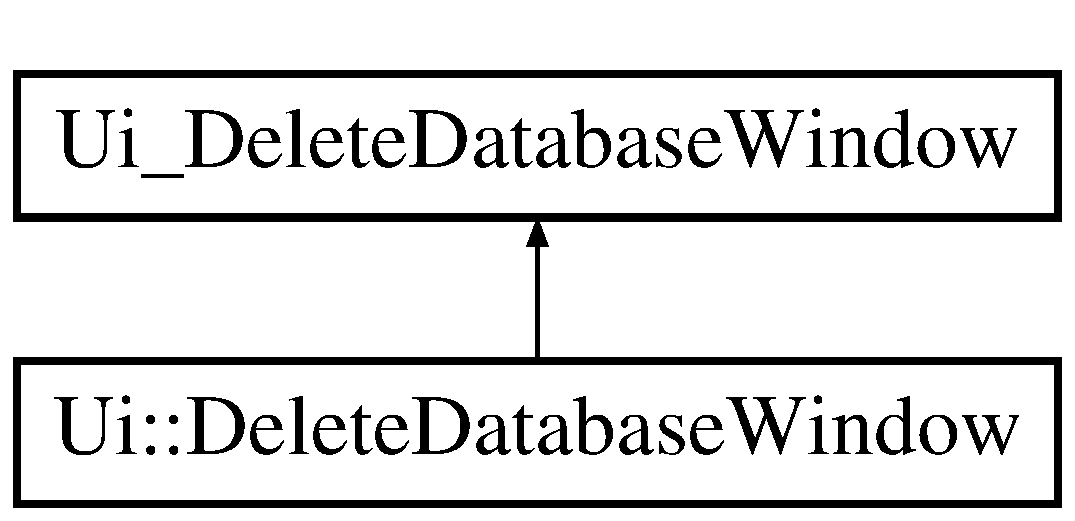
\includegraphics[height=2.000000cm]{class_ui_1_1_delete_database_window}
\end{center}
\end{figure}
\subsection*{Additional Inherited Members}


The documentation for this class was generated from the following file\+:\begin{DoxyCompactItemize}
\item 
ui\+\_\+deletedatabasewindow.\+h\end{DoxyCompactItemize}

\hypertarget{class_dialog}{}\section{Dialog Class Reference}
\label{class_dialog}\index{Dialog@{Dialog}}
Inheritance diagram for Dialog\+:\begin{figure}[H]
\begin{center}
\leavevmode
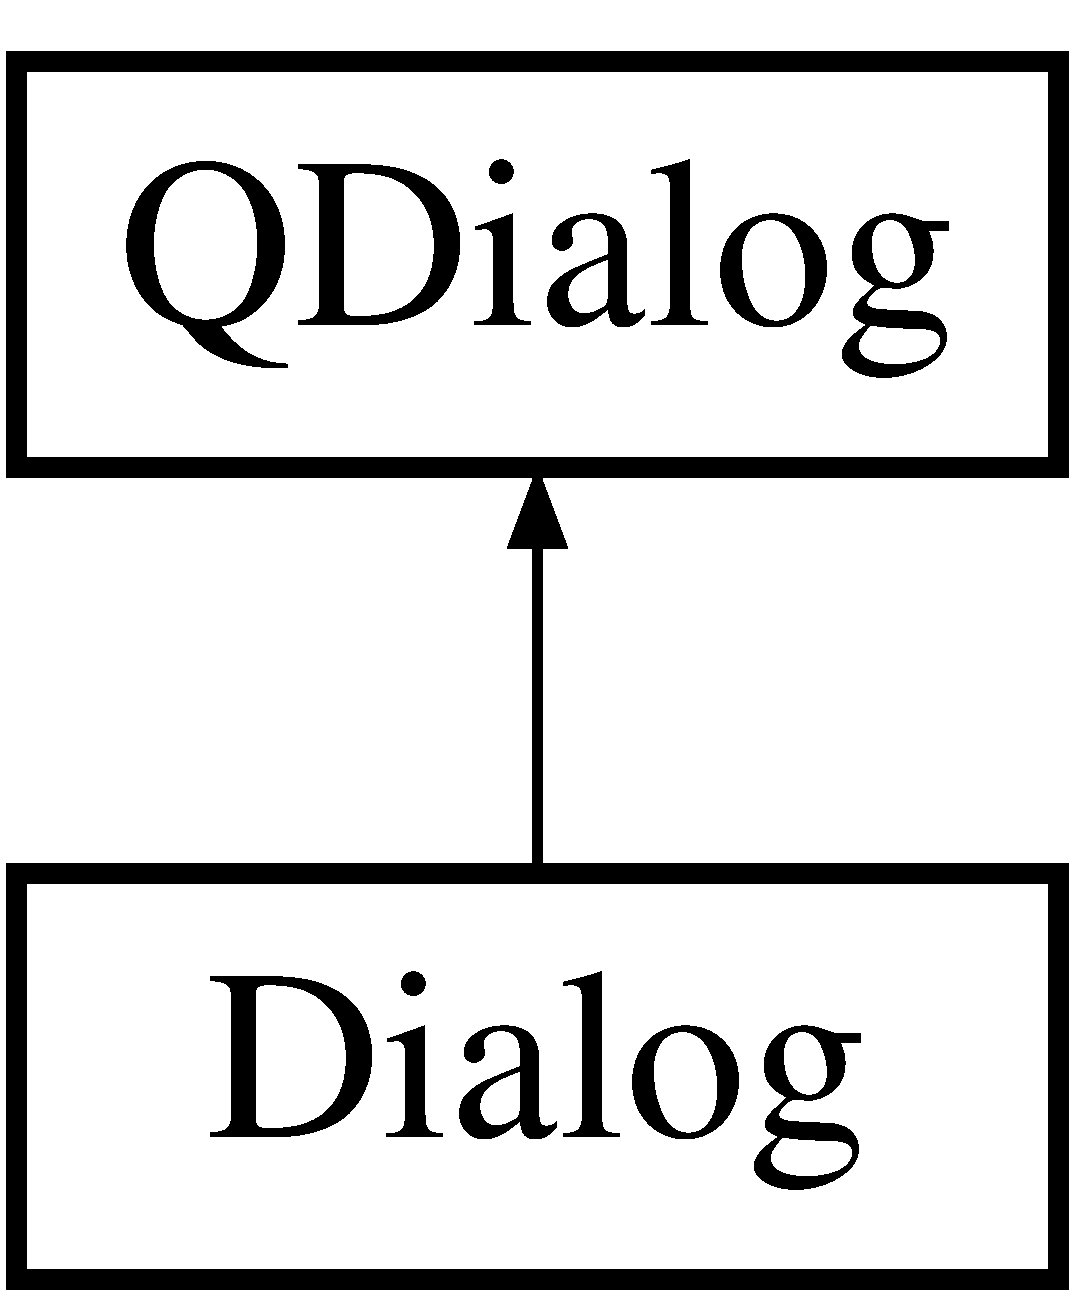
\includegraphics[height=2.000000cm]{class_dialog}
\end{center}
\end{figure}
\subsection*{Public Member Functions}
\begin{DoxyCompactItemize}
\item 
\mbox{\Hypertarget{class_dialog_acfa2063f9f962d394c6a645b6e7e08d8}\label{class_dialog_acfa2063f9f962d394c6a645b6e7e08d8}} 
{\bfseries Dialog} (Q\+Widget $\ast$parent=0)
\end{DoxyCompactItemize}


The documentation for this class was generated from the following files\+:\begin{DoxyCompactItemize}
\item 
dialog.\+h\item 
dialog.\+cpp\end{DoxyCompactItemize}

\hypertarget{class_element}{}\section{Element Class Reference}
\label{class_element}\index{Element@{Element}}


Klasa reprezentująca pojedyńczy element z danej bazy, dostarcza funkcje umożliwiające zarządzanie danym elementem, w tym m.\+in zmianę jego stanu, zwiększenie lub zmniejszenie współczynnika zapamiętania itp.  




{\ttfamily \#include $<$element.\+h$>$}

Inheritance diagram for Element\+:\begin{figure}[H]
\begin{center}
\leavevmode
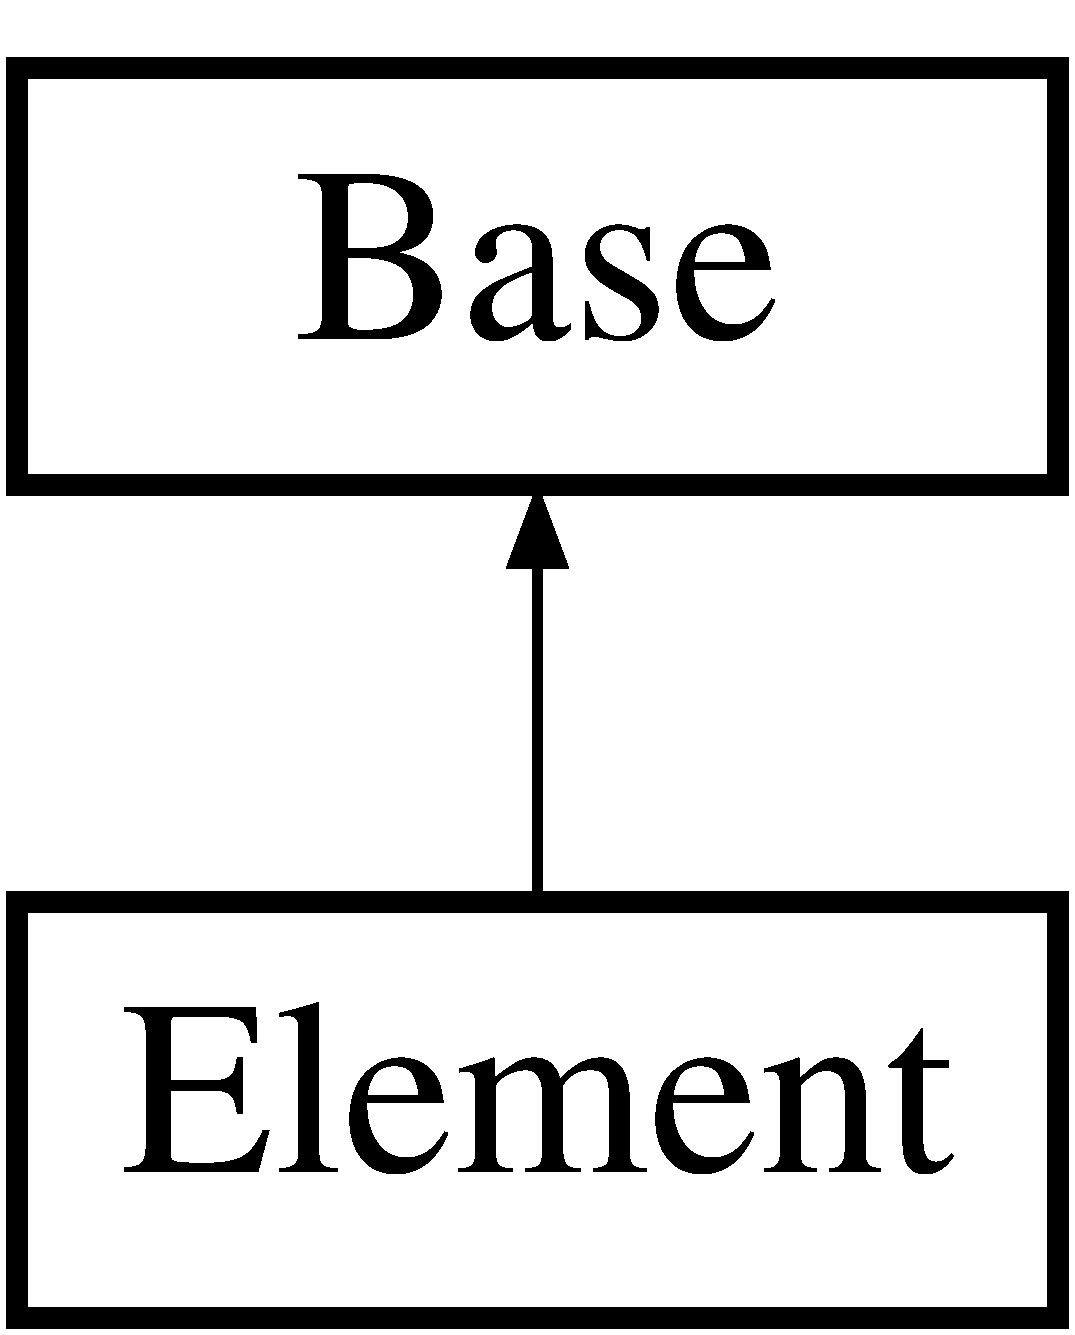
\includegraphics[height=2.000000cm]{class_element}
\end{center}
\end{figure}
\subsection*{Public Member Functions}
\begin{DoxyCompactItemize}
\item 
\mbox{\Hypertarget{class_element_a1c5fd3029cf609e698695b10d3ba9c12}\label{class_element_a1c5fd3029cf609e698695b10d3ba9c12}} 
virtual void {\bfseries import\+Data} (std\+::istream \&in\+\_\+)
\item 
\mbox{\Hypertarget{class_element_aff9d7b31a7aaadafd99d9b3aa1ba1c59}\label{class_element_aff9d7b31a7aaadafd99d9b3aa1ba1c59}} 
virtual void {\bfseries export\+Data} (std\+::ostream \&out\+\_\+)
\item 
\mbox{\Hypertarget{class_element_acb6b4d4a1c3d5b294a1b63ff657d8c4e}\label{class_element_acb6b4d4a1c3d5b294a1b63ff657d8c4e}} 
virtual void {\bfseries add} (\mbox{\hyperlink{class_word}{Word}} word)
\item 
\mbox{\Hypertarget{class_element_a3b2abcbd0a44be55bff0e1d98bbc3f82}\label{class_element_a3b2abcbd0a44be55bff0e1d98bbc3f82}} 
virtual void {\bfseries add} (\mbox{\hyperlink{class_picture}{Picture}} picture)
\item 
\mbox{\Hypertarget{class_element_a992c2fbf75165fcc41e448d73504252d}\label{class_element_a992c2fbf75165fcc41e448d73504252d}} 
virtual void {\bfseries set\+Word} (\mbox{\hyperlink{class_word}{Word}} word)
\item 
\mbox{\Hypertarget{class_element_a4cf241aebdf462dda8aad30a4cc6b4d1}\label{class_element_a4cf241aebdf462dda8aad30a4cc6b4d1}} 
virtual void {\bfseries set\+Picture} (\mbox{\hyperlink{class_picture}{Picture}} word)
\item 
\mbox{\Hypertarget{class_element_ad9ad7d31a3b5f324665ca21d2324c618}\label{class_element_ad9ad7d31a3b5f324665ca21d2324c618}} 
virtual \mbox{\hyperlink{class_word}{Word}} {\bfseries get\+Word} ()
\item 
\mbox{\Hypertarget{class_element_a42ff5b608cea64b46e2e5b1cb21c6892}\label{class_element_a42ff5b608cea64b46e2e5b1cb21c6892}} 
virtual \mbox{\hyperlink{class_picture}{Picture}} {\bfseries get\+Picture} ()
\item 
\mbox{\Hypertarget{class_element_ae74a9371bbbb6444e4b7d001dba56c90}\label{class_element_ae74a9371bbbb6444e4b7d001dba56c90}} 
void {\bfseries increase\+Remembering\+Rate} ()
\item 
\mbox{\Hypertarget{class_element_a9fca38b12a3c6bdda25785e4a34ad9bf}\label{class_element_a9fca38b12a3c6bdda25785e4a34ad9bf}} 
void {\bfseries decrease\+Remembering\+Rate} ()
\item 
\mbox{\Hypertarget{class_element_a02a96acb593527ad29e3eeade4b0db3c}\label{class_element_a02a96acb593527ad29e3eeade4b0db3c}} 
void {\bfseries increase\+Element\+Number} ()
\item 
\mbox{\Hypertarget{class_element_a37a5f4e146bd163265ac635221db0989}\label{class_element_a37a5f4e146bd163265ac635221db0989}} 
void {\bfseries set\+State} ()
\item 
\mbox{\Hypertarget{class_element_a5b9df05146831f5a2ebb4ec2217e4b58}\label{class_element_a5b9df05146831f5a2ebb4ec2217e4b58}} 
void {\bfseries set\+Element\+Number} (unsigned int number)
\item 
\mbox{\Hypertarget{class_element_aa2c0c0905c4b35e907370e7dcb17d58a}\label{class_element_aa2c0c0905c4b35e907370e7dcb17d58a}} 
unsigned int {\bfseries get\+Remembering\+Rate} ()
\item 
\mbox{\Hypertarget{class_element_ac75b3627ff0489f08ffd97c6c2c190bd}\label{class_element_ac75b3627ff0489f08ffd97c6c2c190bd}} 
unsigned int {\bfseries get\+State} ()
\item 
\mbox{\Hypertarget{class_element_afb522900996a2af26c6a5924934532c3}\label{class_element_afb522900996a2af26c6a5924934532c3}} 
unsigned int {\bfseries get\+Element\+Number} ()
\end{DoxyCompactItemize}
\subsection*{Additional Inherited Members}


\subsection{Detailed Description}
Klasa reprezentująca pojedyńczy element z danej bazy, dostarcza funkcje umożliwiające zarządzanie danym elementem, w tym m.\+in zmianę jego stanu, zwiększenie lub zmniejszenie współczynnika zapamiętania itp. 

The documentation for this class was generated from the following files\+:\begin{DoxyCompactItemize}
\item 
element.\+h\item 
element.\+cpp\end{DoxyCompactItemize}

\hypertarget{class_elements_database}{}\section{Elements\+Database Class Reference}
\label{class_elements_database}\index{Elements\+Database@{Elements\+Database}}


Klasa \mbox{\hyperlink{class_elements_database}{Elements\+Database}} reprezentuje daną bazę danych. Przechowuje informacje o bazie oraz jej elementy.  




{\ttfamily \#include $<$elementsdatabase.\+h$>$}

Inheritance diagram for Elements\+Database\+:\begin{figure}[H]
\begin{center}
\leavevmode
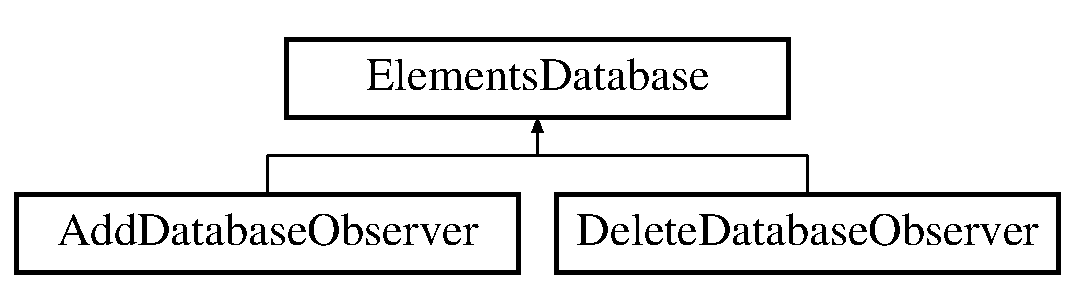
\includegraphics[height=2.000000cm]{class_elements_database}
\end{center}
\end{figure}
\subsection*{Public Member Functions}
\begin{DoxyCompactItemize}
\item 
\mbox{\Hypertarget{class_elements_database_ae370a45ab1134db34ff1a66263d8297b}\label{class_elements_database_ae370a45ab1134db34ff1a66263d8297b}} 
{\bfseries Elements\+Database} (std\+::string database\+\_\+name)
\item 
\mbox{\Hypertarget{class_elements_database_a881af95023218e1382edc0577ec5ef23}\label{class_elements_database_a881af95023218e1382edc0577ec5ef23}} 
virtual void {\bfseries import\+Data} (std\+::istream \&in\+\_\+)
\item 
\mbox{\Hypertarget{class_elements_database_a0aec9b8628c2402a4d78d4be5b3ef6f2}\label{class_elements_database_a0aec9b8628c2402a4d78d4be5b3ef6f2}} 
virtual void {\bfseries export\+Data} (std\+::ostream \&out\+\_\+)
\item 
\mbox{\Hypertarget{class_elements_database_a55558c7804a272361f152dc2e0b3a4c8}\label{class_elements_database_a55558c7804a272361f152dc2e0b3a4c8}} 
virtual void {\bfseries read\+From\+File} ()
\item 
\mbox{\Hypertarget{class_elements_database_a3db3ee74d96dfd50c186588ff578e308}\label{class_elements_database_a3db3ee74d96dfd50c186588ff578e308}} 
virtual void {\bfseries write\+To\+File} ()
\item 
\mbox{\Hypertarget{class_elements_database_a642d59a3e44b0d183523e313065309d4}\label{class_elements_database_a642d59a3e44b0d183523e313065309d4}} 
virtual void {\bfseries read\+Database} ()
\item 
\mbox{\Hypertarget{class_elements_database_a2c18f21690c1b45b37ae825d545a5e36}\label{class_elements_database_a2c18f21690c1b45b37ae825d545a5e36}} 
virtual void {\bfseries write\+Database} ()
\item 
\mbox{\Hypertarget{class_elements_database_ae2c31aa4cb49c37462814fed64aec560}\label{class_elements_database_ae2c31aa4cb49c37462814fed64aec560}} 
virtual void {\bfseries set\+File\+Name} (std\+::string file\+\_\+name)
\item 
\mbox{\Hypertarget{class_elements_database_a8710cd2dad7a2c3c97509daee656f5c6}\label{class_elements_database_a8710cd2dad7a2c3c97509daee656f5c6}} 
virtual void {\bfseries set\+Name} (std\+::string name)
\item 
\mbox{\Hypertarget{class_elements_database_ad2ff356da8d6148ad30b828f91a61605}\label{class_elements_database_ad2ff356da8d6148ad30b828f91a61605}} 
virtual void {\bfseries set\+Default\+File\+Name} ()
\item 
\mbox{\Hypertarget{class_elements_database_a9d070e57b36bd6b95de4fedca69e65de}\label{class_elements_database_a9d070e57b36bd6b95de4fedca69e65de}} 
virtual void {\bfseries swap\+Element} (unsigned int index, \mbox{\hyperlink{class_element}{Element}} new\+\_\+element)
\item 
\mbox{\Hypertarget{class_elements_database_a8bcf9ebeb58a89edb19b4c50fbd8ac3b}\label{class_elements_database_a8bcf9ebeb58a89edb19b4c50fbd8ac3b}} 
virtual void {\bfseries add} (\mbox{\hyperlink{class_element}{Element}} new\+\_\+element)
\item 
\mbox{\Hypertarget{class_elements_database_a28cf4791a1fc0f646b6e3d1d2ccf8c2a}\label{class_elements_database_a28cf4791a1fc0f646b6e3d1d2ccf8c2a}} 
virtual void {\bfseries add} (\mbox{\hyperlink{class_word}{Word}} new\+\_\+element)
\item 
\mbox{\Hypertarget{class_elements_database_acf20ca4257fd66261f2e786a6de10fd9}\label{class_elements_database_acf20ca4257fd66261f2e786a6de10fd9}} 
virtual void {\bfseries add} (\mbox{\hyperlink{class_picture}{Picture}} new\+\_\+element)
\item 
\mbox{\Hypertarget{class_elements_database_a37ffe633a79cf0aa5a30e70fba6945d5}\label{class_elements_database_a37ffe633a79cf0aa5a30e70fba6945d5}} 
virtual std\+::string {\bfseries get\+Default\+File\+Name} ()
\item 
\mbox{\Hypertarget{class_elements_database_ad8f7416174860a5512c6c648d75f65e1}\label{class_elements_database_ad8f7416174860a5512c6c648d75f65e1}} 
void {\bfseries set\+Database} (\mbox{\hyperlink{class_database}{Database}} database)
\item 
\mbox{\Hypertarget{class_elements_database_aef7a58c83877e3eadb67993421c08759}\label{class_elements_database_aef7a58c83877e3eadb67993421c08759}} 
std\+::string {\bfseries get\+Name} ()
\item 
\mbox{\Hypertarget{class_elements_database_a20e9f2279cd9dad94452b011b3a95193}\label{class_elements_database_a20e9f2279cd9dad94452b011b3a95193}} 
std\+::vector$<$ \mbox{\hyperlink{class_element}{Element}} $>$ {\bfseries get\+Elements\+To\+Repeat} ()
\item 
\mbox{\Hypertarget{class_elements_database_aa1580aca3adde71f44987e71b262e031}\label{class_elements_database_aa1580aca3adde71f44987e71b262e031}} 
unsigned int {\bfseries get\+Elements\+To\+Repeat\+Number} ()
\item 
\mbox{\Hypertarget{class_elements_database_abaddac9b4d310335ea2b0736eed31471}\label{class_elements_database_abaddac9b4d310335ea2b0736eed31471}} 
unsigned int {\bfseries get\+Elements\+Number} ()
\item 
\mbox{\Hypertarget{class_elements_database_a911115f8c466c6b4992d6df83182cbb2}\label{class_elements_database_a911115f8c466c6b4992d6df83182cbb2}} 
void {\bfseries swap\+Database\+In\+File} ()
\end{DoxyCompactItemize}
\subsection*{Protected Attributes}
\begin{DoxyCompactItemize}
\item 
\mbox{\Hypertarget{class_elements_database_ab90a3763844239b40a3e6bceafe5651b}\label{class_elements_database_ab90a3763844239b40a3e6bceafe5651b}} 
std\+::vector$<$ \mbox{\hyperlink{class_element}{Element}} $>$ {\bfseries elements\+\_\+}
\item 
\mbox{\Hypertarget{class_elements_database_ad0177aeef6289d365c12a8bbcdfeea37}\label{class_elements_database_ad0177aeef6289d365c12a8bbcdfeea37}} 
\mbox{\hyperlink{class_database}{Database}} {\bfseries database\+\_\+}
\end{DoxyCompactItemize}


\subsection{Detailed Description}
Klasa \mbox{\hyperlink{class_elements_database}{Elements\+Database}} reprezentuje daną bazę danych. Przechowuje informacje o bazie oraz jej elementy. 

The documentation for this class was generated from the following files\+:\begin{DoxyCompactItemize}
\item 
elementsdatabase.\+h\item 
elementsdatabase.\+cpp\end{DoxyCompactItemize}

\hypertarget{class_ui_1_1_get_database_name_window}{}\section{Ui\+:\+:Get\+Database\+Name\+Window Class Reference}
\label{class_ui_1_1_get_database_name_window}\index{Ui\+::\+Get\+Database\+Name\+Window@{Ui\+::\+Get\+Database\+Name\+Window}}
Inheritance diagram for Ui\+:\+:Get\+Database\+Name\+Window\+:\begin{figure}[H]
\begin{center}
\leavevmode
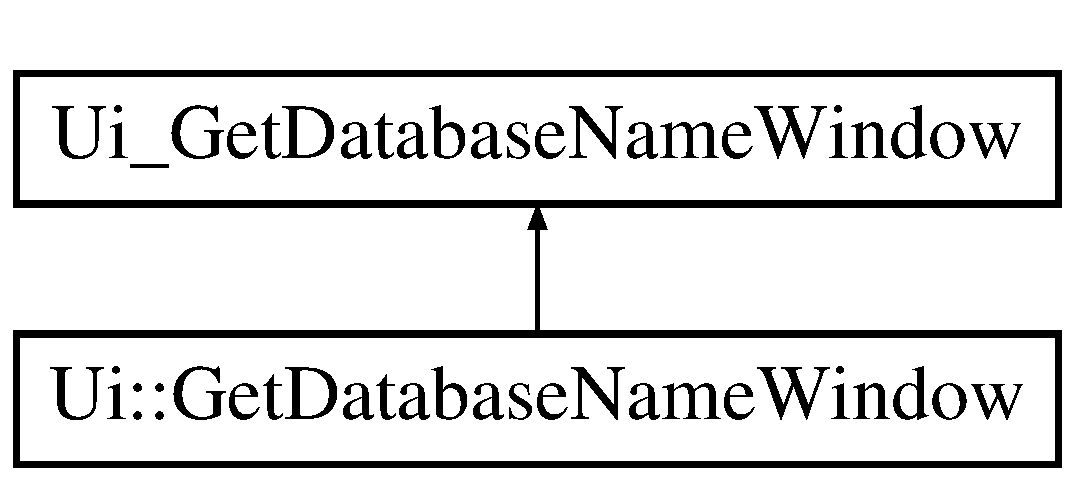
\includegraphics[height=2.000000cm]{class_ui_1_1_get_database_name_window}
\end{center}
\end{figure}
\subsection*{Additional Inherited Members}


The documentation for this class was generated from the following file\+:\begin{DoxyCompactItemize}
\item 
ui\+\_\+getdatabasenamewindow.\+h\end{DoxyCompactItemize}

\hypertarget{class_get_database_name_window}{}\section{Get\+Database\+Name\+Window Class Reference}
\label{class_get_database_name_window}\index{Get\+Database\+Name\+Window@{Get\+Database\+Name\+Window}}


Klasa \mbox{\hyperlink{class_get_database_name_window}{Get\+Database\+Name\+Window}} umożliwia użytkownikowi wpisanie nazwy nowododawanej bazy danych.  




{\ttfamily \#include $<$getdatabasenamewindow.\+h$>$}

Inheritance diagram for Get\+Database\+Name\+Window\+:\begin{figure}[H]
\begin{center}
\leavevmode
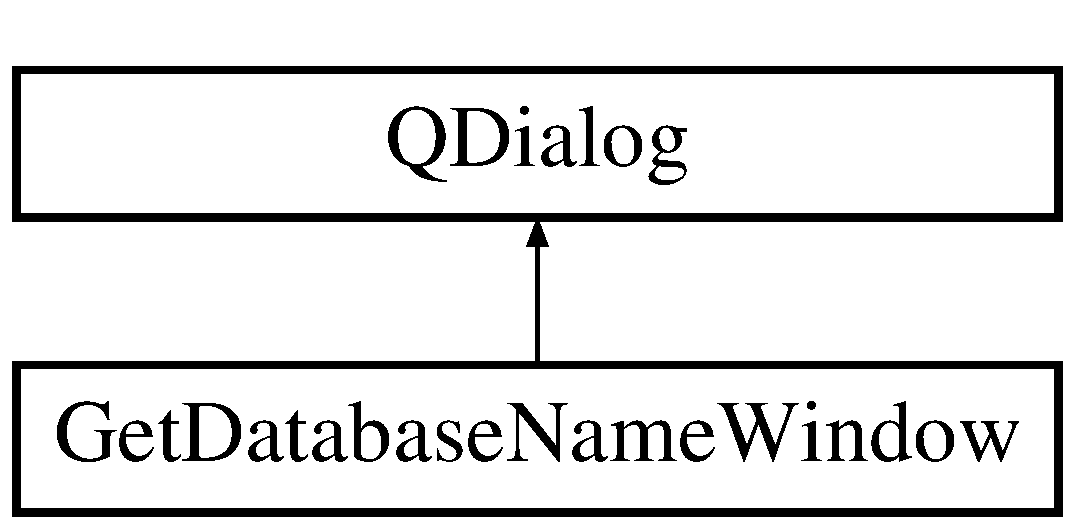
\includegraphics[height=2.000000cm]{class_get_database_name_window}
\end{center}
\end{figure}
\subsection*{Public Member Functions}
\begin{DoxyCompactItemize}
\item 
\mbox{\Hypertarget{class_get_database_name_window_a6d1276a181f974a3c9a899507a6a7485}\label{class_get_database_name_window_a6d1276a181f974a3c9a899507a6a7485}} 
{\bfseries Get\+Database\+Name\+Window} (\mbox{\hyperlink{class_add_database_window}{Add\+Database\+Window}} $\ast$add\+\_\+data\+\_\+window, Q\+Widget $\ast$parent=0, \mbox{\hyperlink{class_menu_start}{Menu\+Start}} $\ast$menu\+\_\+start=0)
\item 
\mbox{\Hypertarget{class_get_database_name_window_adcfec27bffb289f06e18e071e6d87e3d}\label{class_get_database_name_window_adcfec27bffb289f06e18e071e6d87e3d}} 
int {\bfseries show\+Message\+Window} (Q\+String info\+\_\+text)
\item 
\mbox{\Hypertarget{class_get_database_name_window_adca2353140730e90aa481b44de46f94e}\label{class_get_database_name_window_adca2353140730e90aa481b44de46f94e}} 
void {\bfseries do\+Choosen\+Action} (int action)
\end{DoxyCompactItemize}


\subsection{Detailed Description}
Klasa \mbox{\hyperlink{class_get_database_name_window}{Get\+Database\+Name\+Window}} umożliwia użytkownikowi wpisanie nazwy nowododawanej bazy danych. 

The documentation for this class was generated from the following files\+:\begin{DoxyCompactItemize}
\item 
getdatabasenamewindow.\+h\item 
getdatabasenamewindow.\+cpp\end{DoxyCompactItemize}

\hypertarget{class_ui_1_1_main_win}{}\section{Ui\+:\+:Main\+Win Class Reference}
\label{class_ui_1_1_main_win}\index{Ui\+::\+Main\+Win@{Ui\+::\+Main\+Win}}
Inheritance diagram for Ui\+:\+:Main\+Win\+:\begin{figure}[H]
\begin{center}
\leavevmode
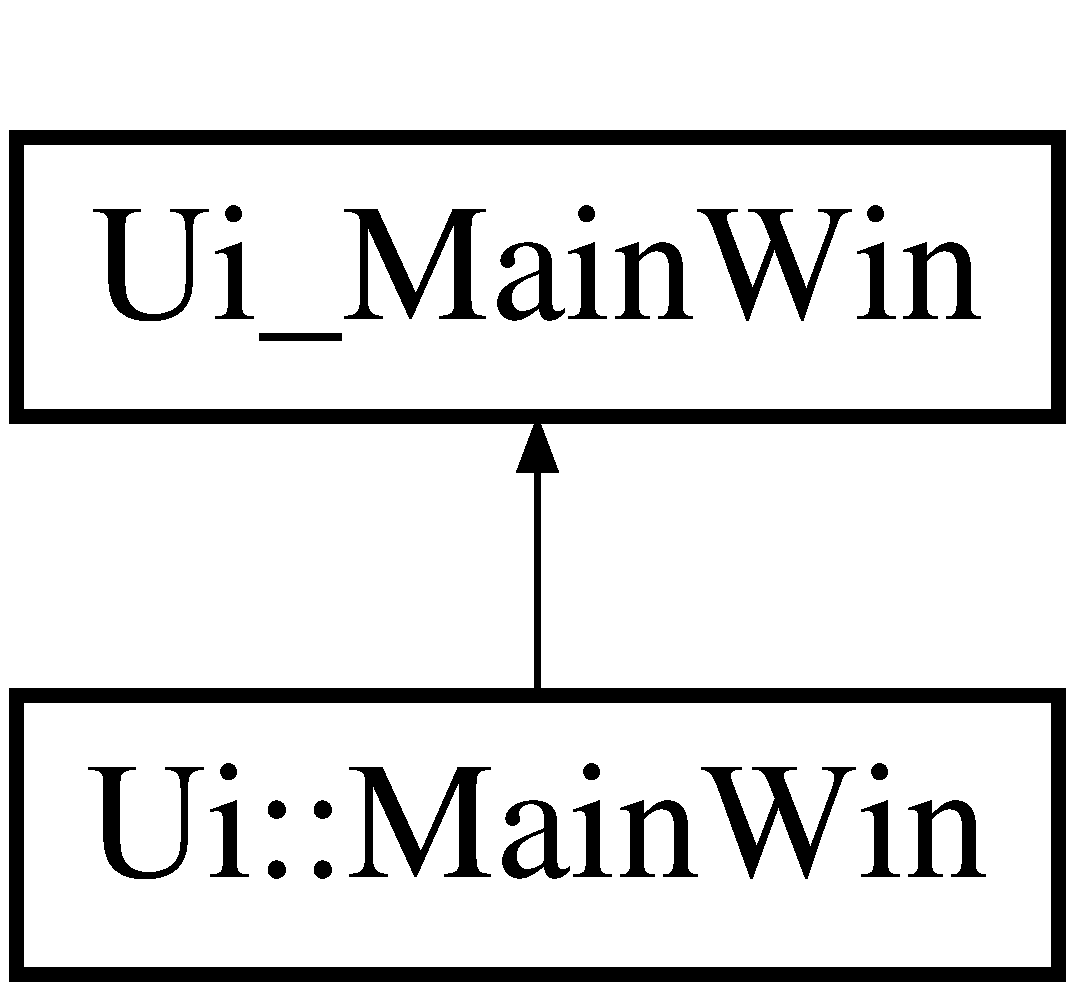
\includegraphics[height=2.000000cm]{class_ui_1_1_main_win}
\end{center}
\end{figure}
\subsection*{Additional Inherited Members}


The documentation for this class was generated from the following file\+:\begin{DoxyCompactItemize}
\item 
ui\+\_\+mainwin.\+h\end{DoxyCompactItemize}

\hypertarget{class_main_win}{}\section{Main\+Win Class Reference}
\label{class_main_win}\index{Main\+Win@{Main\+Win}}


Główne okno programu.  




{\ttfamily \#include $<$mainwin.\+h$>$}

Inheritance diagram for Main\+Win\+:\begin{figure}[H]
\begin{center}
\leavevmode
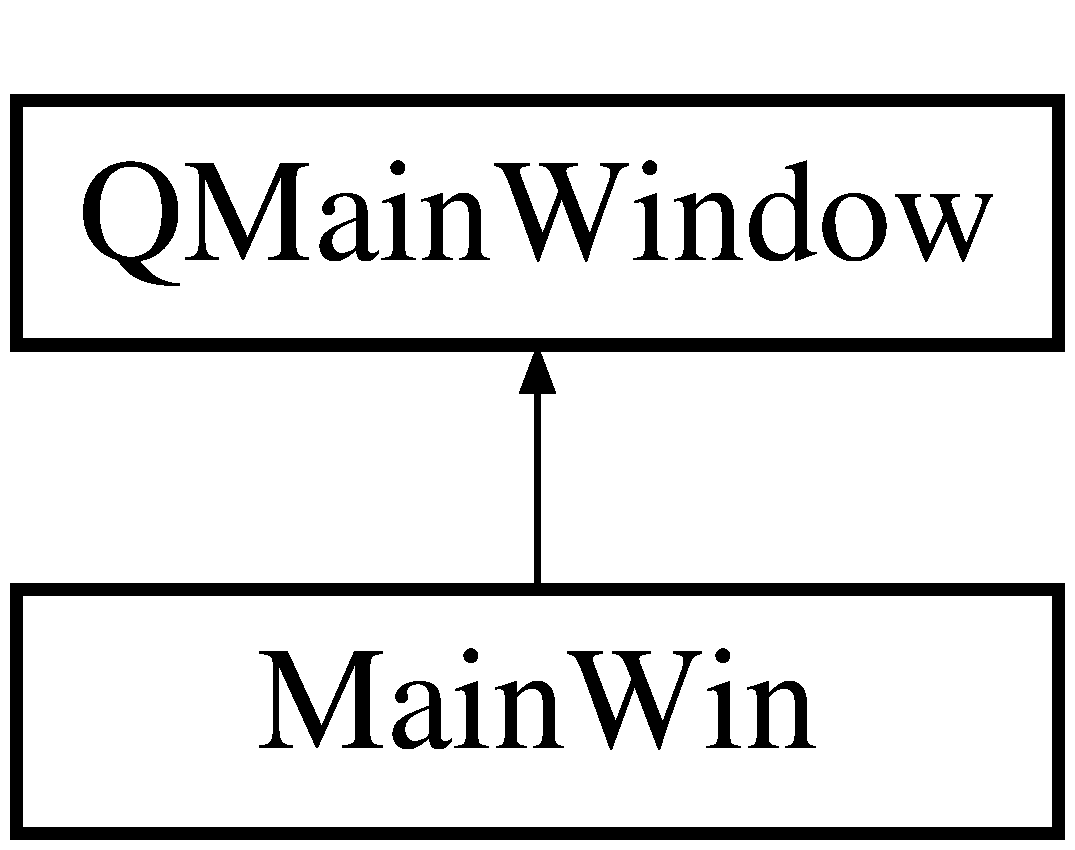
\includegraphics[height=2.000000cm]{class_main_win}
\end{center}
\end{figure}
\subsection*{Public Member Functions}
\begin{DoxyCompactItemize}
\item 
\mbox{\Hypertarget{class_main_win_a6b5f1fb3c79f705570e57c1838ccb2e9}\label{class_main_win_a6b5f1fb3c79f705570e57c1838ccb2e9}} 
{\bfseries Main\+Win} (Q\+Widget $\ast$parent=0, \mbox{\hyperlink{class_menu_start}{Menu\+Start}} $\ast$win=0)
\item 
\mbox{\Hypertarget{class_main_win_a927f5e011ea2c3eef5a112173c693029}\label{class_main_win_a927f5e011ea2c3eef5a112173c693029}} 
void {\bfseries set\+Repetition} (Q\+String name)
\item 
\mbox{\Hypertarget{class_main_win_aed160d223350e6b9c0a74c4be1108b09}\label{class_main_win_aed160d223350e6b9c0a74c4be1108b09}} 
void {\bfseries show\+Element} ()
\item 
\mbox{\Hypertarget{class_main_win_ade439601c33cfd33472ea9c9f87017db}\label{class_main_win_ade439601c33cfd33472ea9c9f87017db}} 
int {\bfseries get\+State} ()
\item 
\mbox{\Hypertarget{class_main_win_aa3280cf1c23f3b578a0acb486a23d989}\label{class_main_win_aa3280cf1c23f3b578a0acb486a23d989}} 
int {\bfseries show\+Message\+Window} (Q\+String info\+\_\+text)
\item 
\mbox{\Hypertarget{class_main_win_ad23b2f0e0498b3d42b6ac35091cc771f}\label{class_main_win_ad23b2f0e0498b3d42b6ac35091cc771f}} 
void {\bfseries do\+Choosen\+Action} (int action)
\item 
\mbox{\Hypertarget{class_main_win_a944961976d6b9b6692f6e09afb20edee}\label{class_main_win_a944961976d6b9b6692f6e09afb20edee}} 
void {\bfseries show\+Details} ()
\end{DoxyCompactItemize}


\subsection{Detailed Description}
Główne okno programu. 

The documentation for this class was generated from the following files\+:\begin{DoxyCompactItemize}
\item 
mainwin.\+h\item 
mainwin.\+cpp\end{DoxyCompactItemize}

\hypertarget{class_ui_1_1_menu_start}{}\section{Ui\+:\+:Menu\+Start Class Reference}
\label{class_ui_1_1_menu_start}\index{Ui\+::\+Menu\+Start@{Ui\+::\+Menu\+Start}}
Inheritance diagram for Ui\+:\+:Menu\+Start\+:\begin{figure}[H]
\begin{center}
\leavevmode
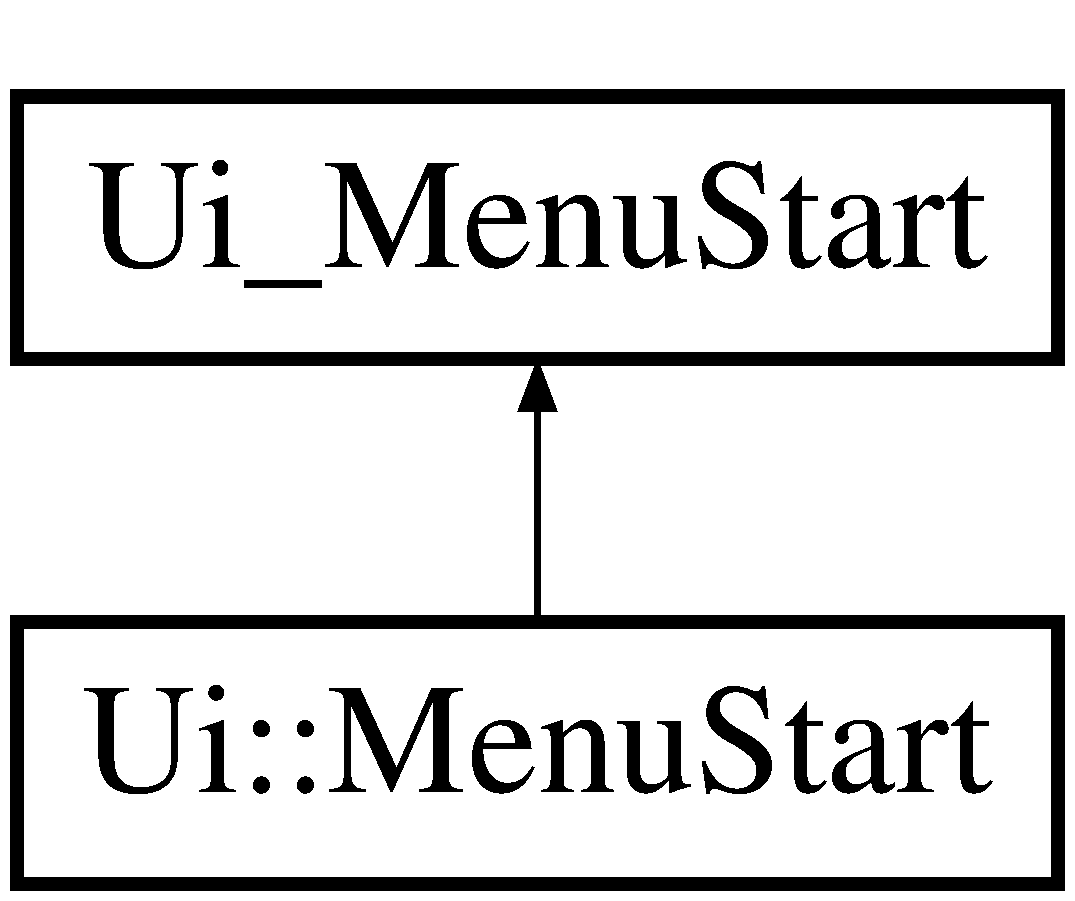
\includegraphics[height=2.000000cm]{class_ui_1_1_menu_start}
\end{center}
\end{figure}
\subsection*{Additional Inherited Members}


The documentation for this class was generated from the following file\+:\begin{DoxyCompactItemize}
\item 
ui\+\_\+menustart.\+h\end{DoxyCompactItemize}

\hypertarget{class_menu_start}{}\section{Menu\+Start Class Reference}
\label{class_menu_start}\index{Menu\+Start@{Menu\+Start}}


Klasam reprezentuje okno startowe, umożliwia użytkowi wybranie konkretnych akcji.  




{\ttfamily \#include $<$menustart.\+h$>$}

Inheritance diagram for Menu\+Start\+:\begin{figure}[H]
\begin{center}
\leavevmode
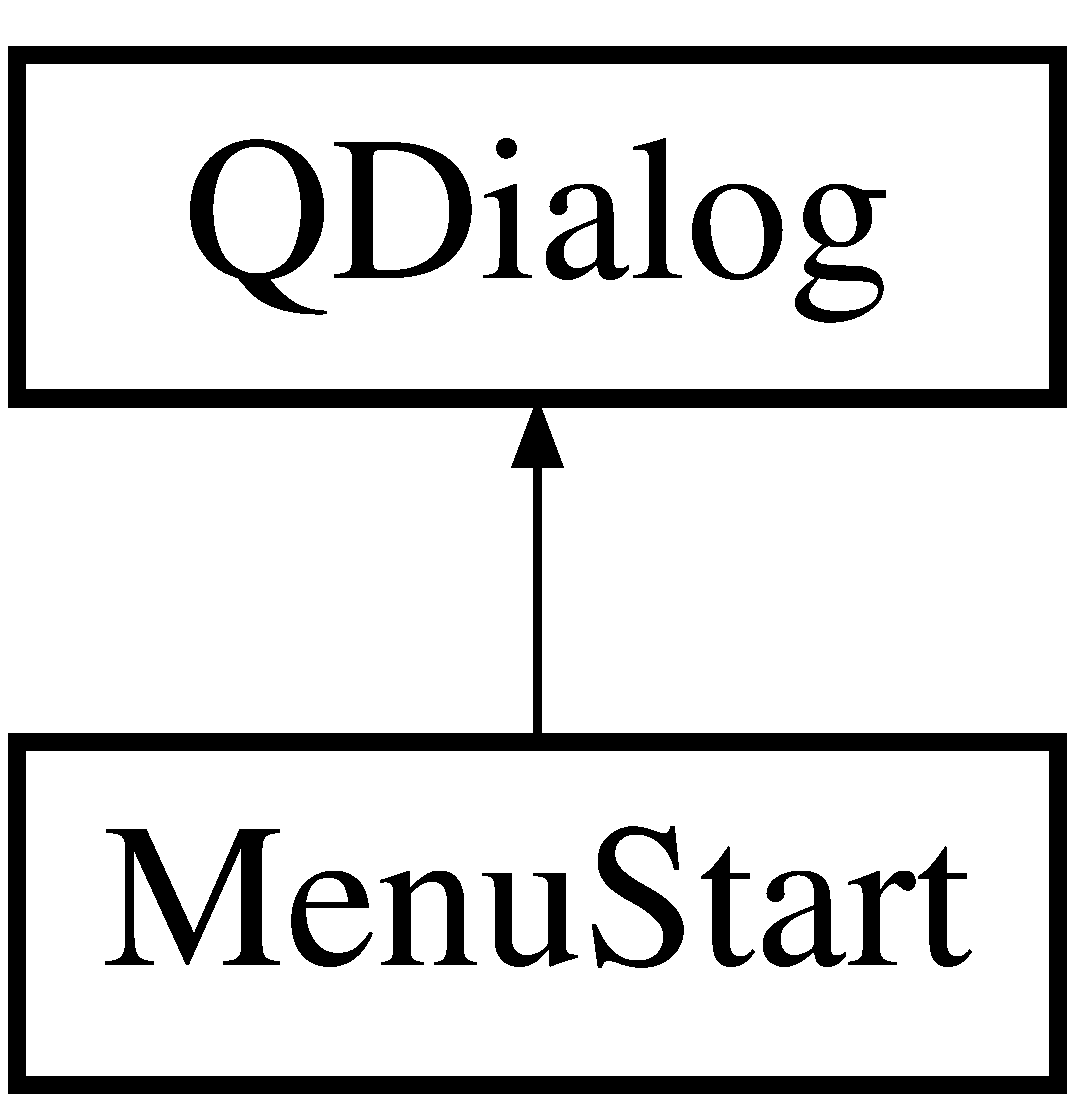
\includegraphics[height=2.000000cm]{class_menu_start}
\end{center}
\end{figure}
\subsection*{Public Member Functions}
\begin{DoxyCompactItemize}
\item 
\mbox{\Hypertarget{class_menu_start_a184ff65bb2534378670fee22487b02eb}\label{class_menu_start_a184ff65bb2534378670fee22487b02eb}} 
{\bfseries Menu\+Start} (Q\+Widget $\ast$parent=0)
\item 
\mbox{\Hypertarget{class_menu_start_a52634af21c3f1c8fc71c202d9618dab3}\label{class_menu_start_a52634af21c3f1c8fc71c202d9618dab3}} 
void {\bfseries set\+Database\+Name} (std\+::string name)
\end{DoxyCompactItemize}


\subsection{Detailed Description}
Klasam reprezentuje okno startowe, umożliwia użytkowi wybranie konkretnych akcji. 

The documentation for this class was generated from the following files\+:\begin{DoxyCompactItemize}
\item 
menustart.\+h\item 
menustart.\+cpp\end{DoxyCompactItemize}

\hypertarget{class_picture}{}\section{Picture Class Reference}
\label{class_picture}\index{Picture@{Picture}}


Klasa przechowuje informacje o obrazku dołączonym do danego elementu.  




{\ttfamily \#include $<$picture.\+h$>$}

Inheritance diagram for Picture\+:\begin{figure}[H]
\begin{center}
\leavevmode
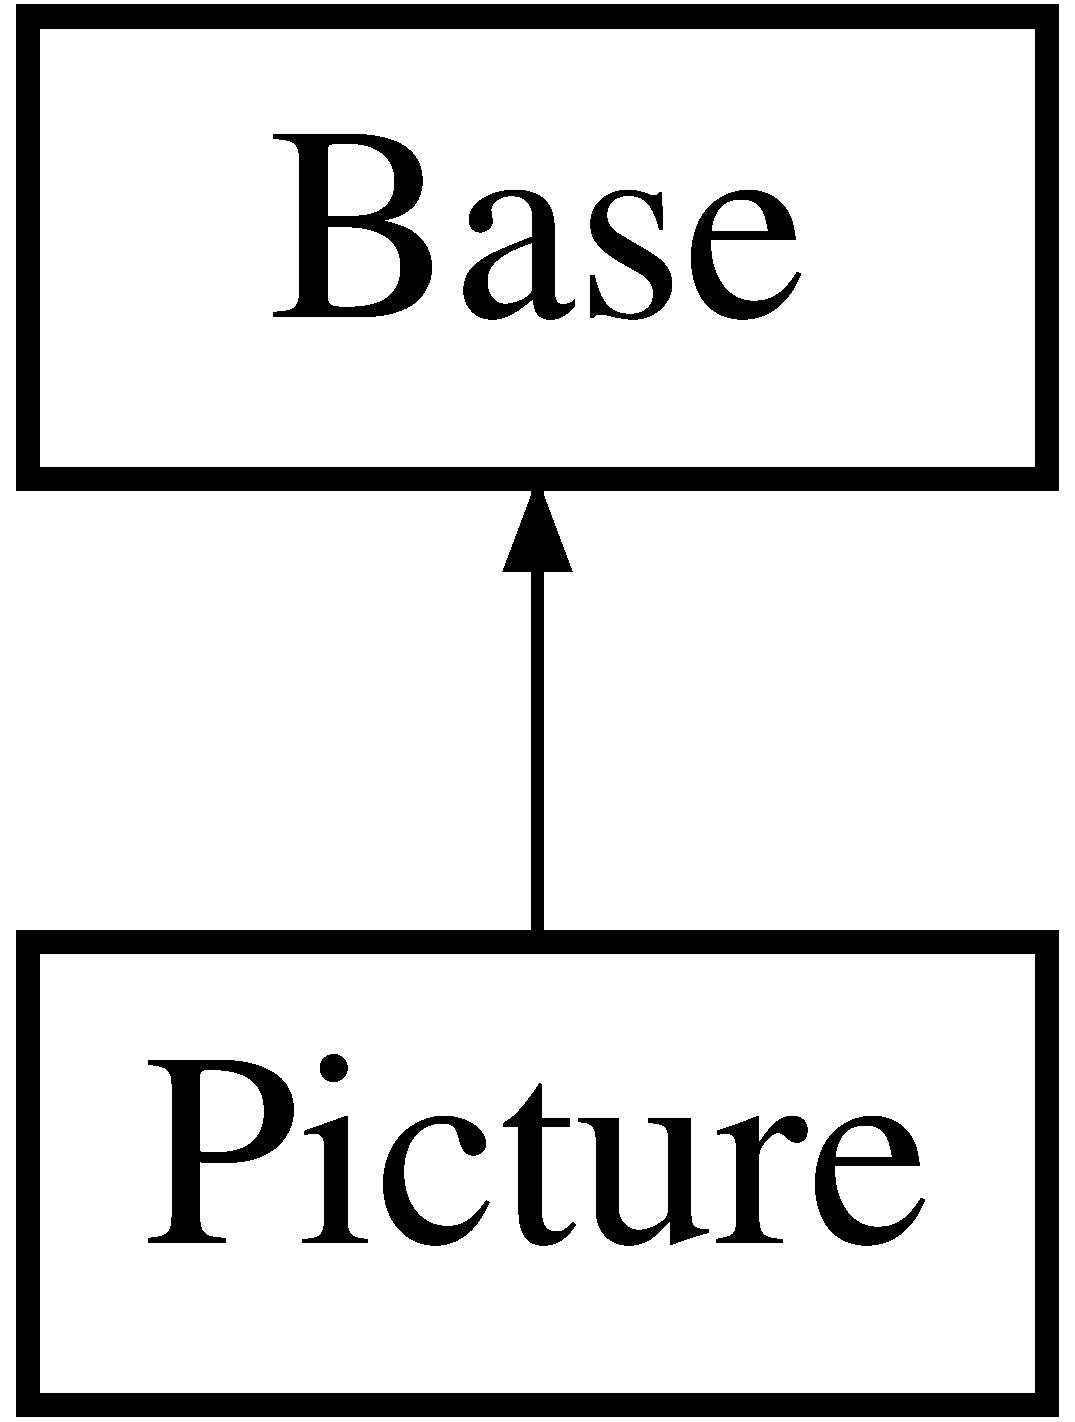
\includegraphics[height=2.000000cm]{class_picture}
\end{center}
\end{figure}
\subsection*{Public Member Functions}
\begin{DoxyCompactItemize}
\item 
\mbox{\Hypertarget{class_picture_afaa06c0b911691026417379d5b78477d}\label{class_picture_afaa06c0b911691026417379d5b78477d}} 
virtual void {\bfseries import\+Data} (std\+::istream \&in\+\_\+)
\item 
\mbox{\Hypertarget{class_picture_a38c495d9851a7ebe12344d7b8e7075d5}\label{class_picture_a38c495d9851a7ebe12344d7b8e7075d5}} 
virtual void {\bfseries export\+Data} (std\+::ostream \&out\+\_\+)
\item 
\mbox{\Hypertarget{class_picture_a8826800da424208a9475242817c2d050}\label{class_picture_a8826800da424208a9475242817c2d050}} 
virtual void {\bfseries set\+Path} (std\+::string path)
\item 
\mbox{\Hypertarget{class_picture_ac9f36933f7bf3ac9e40684891b2129bb}\label{class_picture_ac9f36933f7bf3ac9e40684891b2129bb}} 
virtual std\+::string {\bfseries get\+Path} ()
\item 
\mbox{\Hypertarget{class_picture_a128bb0b00a4d0b0685bedb00160e3991}\label{class_picture_a128bb0b00a4d0b0685bedb00160e3991}} 
virtual void {\bfseries add} (\mbox{\hyperlink{class_base}{Base}} $\ast$)
\end{DoxyCompactItemize}
\subsection*{Additional Inherited Members}


\subsection{Detailed Description}
Klasa przechowuje informacje o obrazku dołączonym do danego elementu. 

The documentation for this class was generated from the following files\+:\begin{DoxyCompactItemize}
\item 
picture.\+h\item 
picture.\+cpp\end{DoxyCompactItemize}

\hypertarget{class_repetition}{}\section{Repetition Class Reference}
\label{class_repetition}\index{Repetition@{Repetition}}


Klasa reprezentuje aktualna powtórkę, przechowuje tylko te elementy danej bazy które należy powtórzyć w danym dniu. Umożliwia kolejne wyświetlanie elementów w głownym oknie programu.  




{\ttfamily \#include $<$repetition.\+h$>$}

\subsection*{Public Member Functions}
\begin{DoxyCompactItemize}
\item 
\mbox{\Hypertarget{class_repetition_a090f29e6791686f98f97d08aecd3e73f}\label{class_repetition_a090f29e6791686f98f97d08aecd3e73f}} 
{\bfseries Repetition} (std\+::string database\+\_\+name)
\item 
\mbox{\Hypertarget{class_repetition_ac4fc496f123f6889987b2fc1cc2cd6bc}\label{class_repetition_ac4fc496f123f6889987b2fc1cc2cd6bc}} 
void {\bfseries set\+Current\+Repetitions} ()
\item 
\mbox{\Hypertarget{class_repetition_ab0c80b930deaa082d58de162c94171ad}\label{class_repetition_ab0c80b930deaa082d58de162c94171ad}} 
void {\bfseries save\+Repetition} ()
\item 
\mbox{\Hypertarget{class_repetition_ad7a38b006f3bea43c1e078c18696cd5a}\label{class_repetition_ad7a38b006f3bea43c1e078c18696cd5a}} 
int {\bfseries get\+State} ()
\item 
\mbox{\Hypertarget{class_repetition_a17b859f4c0018687e10c1a1f9fc73058}\label{class_repetition_a17b859f4c0018687e10c1a1f9fc73058}} 
int {\bfseries get\+Repetitions\+Number} ()
\item 
\mbox{\Hypertarget{class_repetition_a61e44eaf56509396ab0f84f4a8b9dba6}\label{class_repetition_a61e44eaf56509396ab0f84f4a8b9dba6}} 
std\+::vector$<$ \mbox{\hyperlink{class_element}{Element}} $>$\+::iterator {\bfseries get\+Current\+Repetitions} ()
\item 
\mbox{\Hypertarget{class_repetition_a6771c9a3a6800aa96ef3a1b57cc4f46b}\label{class_repetition_a6771c9a3a6800aa96ef3a1b57cc4f46b}} 
std\+::vector$<$ \mbox{\hyperlink{class_element}{Element}} $>$\+::iterator {\bfseries get\+End\+Iterator} ()
\item 
\mbox{\Hypertarget{class_repetition_af6b10b986daed2831410200fafb44115}\label{class_repetition_af6b10b986daed2831410200fafb44115}} 
std\+::string {\bfseries get\+Current\+Database} ()
\end{DoxyCompactItemize}


\subsection{Detailed Description}
Klasa reprezentuje aktualna powtórkę, przechowuje tylko te elementy danej bazy które należy powtórzyć w danym dniu. Umożliwia kolejne wyświetlanie elementów w głownym oknie programu. 

The documentation for this class was generated from the following files\+:\begin{DoxyCompactItemize}
\item 
repetition.\+h\item 
repetition.\+cpp\end{DoxyCompactItemize}

\hypertarget{class_ui___add_database_window}{}\section{Ui\+\_\+\+Add\+Database\+Window Class Reference}
\label{class_ui___add_database_window}\index{Ui\+\_\+\+Add\+Database\+Window@{Ui\+\_\+\+Add\+Database\+Window}}
Inheritance diagram for Ui\+\_\+\+Add\+Database\+Window\+:\begin{figure}[H]
\begin{center}
\leavevmode
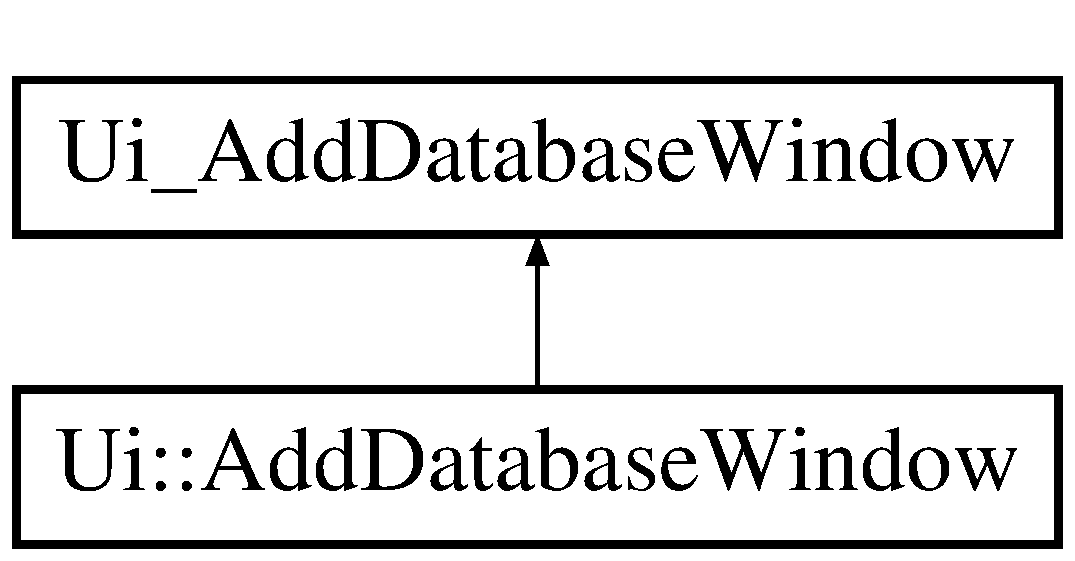
\includegraphics[height=2.000000cm]{class_ui___add_database_window}
\end{center}
\end{figure}
\subsection*{Public Member Functions}
\begin{DoxyCompactItemize}
\item 
\mbox{\Hypertarget{class_ui___add_database_window_a7907700637591b9da392ef46548df7d7}\label{class_ui___add_database_window_a7907700637591b9da392ef46548df7d7}} 
void {\bfseries setup\+Ui} (Q\+Widget $\ast$\mbox{\hyperlink{class_add_database_window}{Add\+Database\+Window}})
\item 
\mbox{\Hypertarget{class_ui___add_database_window_a905d92efe4020e6450f67a8db8ea8a96}\label{class_ui___add_database_window_a905d92efe4020e6450f67a8db8ea8a96}} 
void {\bfseries retranslate\+Ui} (Q\+Widget $\ast$\mbox{\hyperlink{class_add_database_window}{Add\+Database\+Window}})
\end{DoxyCompactItemize}
\subsection*{Public Attributes}
\begin{DoxyCompactItemize}
\item 
\mbox{\Hypertarget{class_ui___add_database_window_afbfd0e2583733aaae4050194f30bcb2f}\label{class_ui___add_database_window_afbfd0e2583733aaae4050194f30bcb2f}} 
Q\+Widget $\ast$ {\bfseries vertical\+Layout\+Widget}
\item 
\mbox{\Hypertarget{class_ui___add_database_window_aa939a3c35e7d6292163e1c6d75df4cac}\label{class_ui___add_database_window_aa939a3c35e7d6292163e1c6d75df4cac}} 
Q\+V\+Box\+Layout $\ast$ {\bfseries vertical\+Layout}
\item 
\mbox{\Hypertarget{class_ui___add_database_window_a5e06e2e185e11a46cd4b5dfe5f637a8e}\label{class_ui___add_database_window_a5e06e2e185e11a46cd4b5dfe5f637a8e}} 
Q\+Push\+Button $\ast$ {\bfseries push\+Button\+\_\+2}
\item 
\mbox{\Hypertarget{class_ui___add_database_window_ab6021e38debe488f6186376d9c69800e}\label{class_ui___add_database_window_ab6021e38debe488f6186376d9c69800e}} 
Q\+Push\+Button $\ast$ {\bfseries push\+Button}
\item 
\mbox{\Hypertarget{class_ui___add_database_window_a031c028b8ba1bccb2ab15396a29e0e22}\label{class_ui___add_database_window_a031c028b8ba1bccb2ab15396a29e0e22}} 
Q\+Label $\ast$ {\bfseries label}
\item 
\mbox{\Hypertarget{class_ui___add_database_window_aeaf7e4455c123591cb7c54cf16483342}\label{class_ui___add_database_window_aeaf7e4455c123591cb7c54cf16483342}} 
Q\+Label $\ast$ {\bfseries label\+\_\+2}
\item 
\mbox{\Hypertarget{class_ui___add_database_window_a7478dd17396fa863f394b30183489057}\label{class_ui___add_database_window_a7478dd17396fa863f394b30183489057}} 
Q\+Line\+Edit $\ast$ {\bfseries line\+Edit}
\item 
\mbox{\Hypertarget{class_ui___add_database_window_a982098dd008de01be5b312c164c59b85}\label{class_ui___add_database_window_a982098dd008de01be5b312c164c59b85}} 
Q\+Line\+Edit $\ast$ {\bfseries line\+Edit\+\_\+2}
\item 
\mbox{\Hypertarget{class_ui___add_database_window_a00c531b02fdd0feb2f7ea5015ddb8577}\label{class_ui___add_database_window_a00c531b02fdd0feb2f7ea5015ddb8577}} 
Q\+Plain\+Text\+Edit $\ast$ {\bfseries plain\+Text\+Edit}
\item 
\mbox{\Hypertarget{class_ui___add_database_window_ab3410335b4951e5071ba0a5efb8c865b}\label{class_ui___add_database_window_ab3410335b4951e5071ba0a5efb8c865b}} 
Q\+Label $\ast$ {\bfseries label\+\_\+3}
\item 
\mbox{\Hypertarget{class_ui___add_database_window_aaf675288c2490619b8e27eb50f086d5c}\label{class_ui___add_database_window_aaf675288c2490619b8e27eb50f086d5c}} 
Q\+Label $\ast$ {\bfseries label\+\_\+4}
\item 
\mbox{\Hypertarget{class_ui___add_database_window_a920969352e23c5287b4eb30301a4935c}\label{class_ui___add_database_window_a920969352e23c5287b4eb30301a4935c}} 
Q\+Push\+Button $\ast$ {\bfseries choose\+\_\+picture\+\_\+button}
\item 
\mbox{\Hypertarget{class_ui___add_database_window_a81c579e917bee2c70f6b61421a5854c0}\label{class_ui___add_database_window_a81c579e917bee2c70f6b61421a5854c0}} 
Q\+Label $\ast$ {\bfseries image\+\_\+label}
\end{DoxyCompactItemize}


The documentation for this class was generated from the following file\+:\begin{DoxyCompactItemize}
\item 
ui\+\_\+adddatabasewindow.\+h\end{DoxyCompactItemize}

\hypertarget{class_ui___choose_database_window}{}\section{Ui\+\_\+\+Choose\+Database\+Window Class Reference}
\label{class_ui___choose_database_window}\index{Ui\+\_\+\+Choose\+Database\+Window@{Ui\+\_\+\+Choose\+Database\+Window}}
Inheritance diagram for Ui\+\_\+\+Choose\+Database\+Window\+:\begin{figure}[H]
\begin{center}
\leavevmode
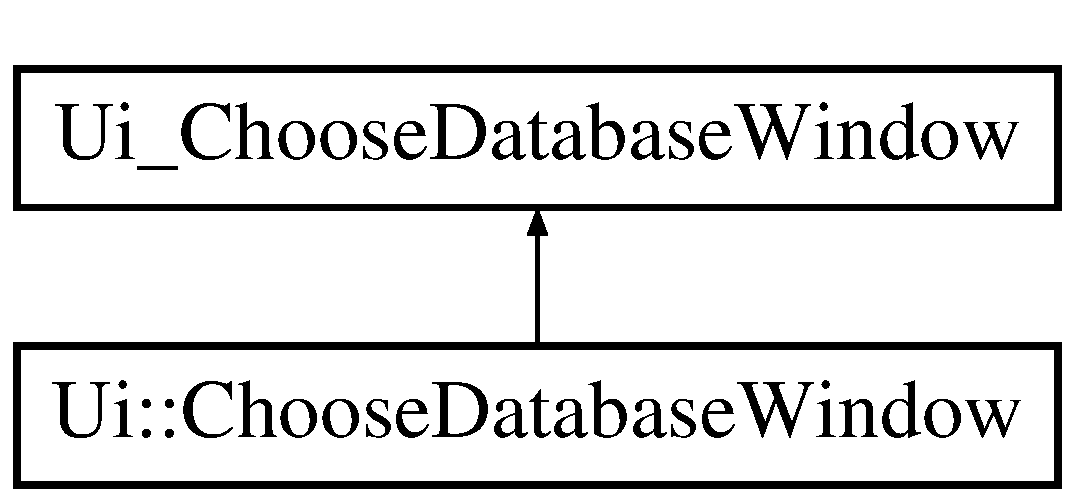
\includegraphics[height=2.000000cm]{class_ui___choose_database_window}
\end{center}
\end{figure}
\subsection*{Public Member Functions}
\begin{DoxyCompactItemize}
\item 
\mbox{\Hypertarget{class_ui___choose_database_window_a00855a927ef06e319c7fefefd7aad3a8}\label{class_ui___choose_database_window_a00855a927ef06e319c7fefefd7aad3a8}} 
void {\bfseries setup\+Ui} (Q\+Widget $\ast$\mbox{\hyperlink{class_choose_database_window}{Choose\+Database\+Window}})
\item 
\mbox{\Hypertarget{class_ui___choose_database_window_a7f26434d7baa953de715b029e36defbf}\label{class_ui___choose_database_window_a7f26434d7baa953de715b029e36defbf}} 
void {\bfseries retranslate\+Ui} (Q\+Widget $\ast$\mbox{\hyperlink{class_choose_database_window}{Choose\+Database\+Window}})
\end{DoxyCompactItemize}
\subsection*{Public Attributes}
\begin{DoxyCompactItemize}
\item 
\mbox{\Hypertarget{class_ui___choose_database_window_a6e6c277700117e6398586d2a5649e36c}\label{class_ui___choose_database_window_a6e6c277700117e6398586d2a5649e36c}} 
Q\+Widget $\ast$ {\bfseries grid\+Layout\+Widget}
\item 
\mbox{\Hypertarget{class_ui___choose_database_window_ac90ea77e8a617a76bb7fab6959489b7c}\label{class_ui___choose_database_window_ac90ea77e8a617a76bb7fab6959489b7c}} 
Q\+Grid\+Layout $\ast$ {\bfseries grid\+Layout}
\item 
\mbox{\Hypertarget{class_ui___choose_database_window_ac987b0a090ee4e8cd28df3d35e81a646}\label{class_ui___choose_database_window_ac987b0a090ee4e8cd28df3d35e81a646}} 
Q\+Push\+Button $\ast$ {\bfseries exit\+\_\+button}
\item 
\mbox{\Hypertarget{class_ui___choose_database_window_a3e74e982c89730bd9f8c722ce7c89f0d}\label{class_ui___choose_database_window_a3e74e982c89730bd9f8c722ce7c89f0d}} 
Q\+Push\+Button $\ast$ {\bfseries save\+\_\+button}
\item 
\mbox{\Hypertarget{class_ui___choose_database_window_a3738b8edeae045577cffd76af84d4d48}\label{class_ui___choose_database_window_a3738b8edeae045577cffd76af84d4d48}} 
Q\+Scroll\+Area $\ast$ {\bfseries scroll\+Area}
\item 
\mbox{\Hypertarget{class_ui___choose_database_window_ac800d1c4c43bc2d9fa6d78d748d9d08a}\label{class_ui___choose_database_window_ac800d1c4c43bc2d9fa6d78d748d9d08a}} 
Q\+Widget $\ast$ {\bfseries scroll\+Area\+Widget\+Contents}
\item 
\mbox{\Hypertarget{class_ui___choose_database_window_a948771d06f7c81857279cf06d27bd571}\label{class_ui___choose_database_window_a948771d06f7c81857279cf06d27bd571}} 
Q\+List\+View $\ast$ {\bfseries list\+View}
\item 
\mbox{\Hypertarget{class_ui___choose_database_window_ad4570e7601f2f3826f9b80415a913d40}\label{class_ui___choose_database_window_ad4570e7601f2f3826f9b80415a913d40}} 
Q\+Slider $\ast$ {\bfseries vertical\+Slider}
\item 
\mbox{\Hypertarget{class_ui___choose_database_window_ab05ca5555ee78080d494531311e22d4f}\label{class_ui___choose_database_window_ab05ca5555ee78080d494531311e22d4f}} 
Q\+Scroll\+Bar $\ast$ {\bfseries vertical\+Scroll\+Bar}
\item 
\mbox{\Hypertarget{class_ui___choose_database_window_a42454f18842284f769d3c70f38f04a74}\label{class_ui___choose_database_window_a42454f18842284f769d3c70f38f04a74}} 
Q\+Label $\ast$ {\bfseries image\+\_\+label}
\end{DoxyCompactItemize}


The documentation for this class was generated from the following file\+:\begin{DoxyCompactItemize}
\item 
ui\+\_\+choosedatabasewindow.\+h\end{DoxyCompactItemize}

\hypertarget{class_ui___delete_database_window}{}\section{Ui\+\_\+\+Delete\+Database\+Window Class Reference}
\label{class_ui___delete_database_window}\index{Ui\+\_\+\+Delete\+Database\+Window@{Ui\+\_\+\+Delete\+Database\+Window}}
Inheritance diagram for Ui\+\_\+\+Delete\+Database\+Window\+:\begin{figure}[H]
\begin{center}
\leavevmode
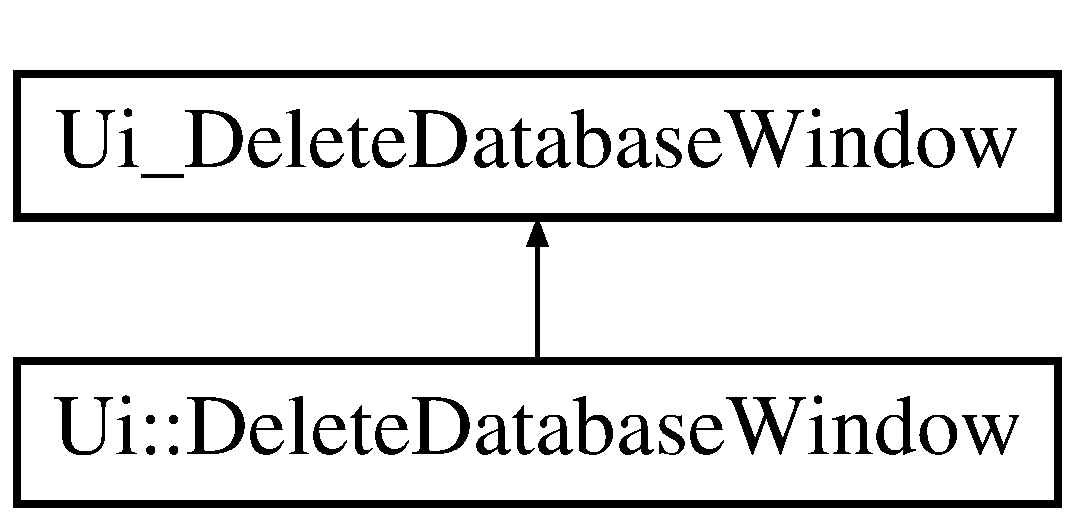
\includegraphics[height=2.000000cm]{class_ui___delete_database_window}
\end{center}
\end{figure}
\subsection*{Public Member Functions}
\begin{DoxyCompactItemize}
\item 
\mbox{\Hypertarget{class_ui___delete_database_window_a74620a9727fa723b177d0b1f3b336c05}\label{class_ui___delete_database_window_a74620a9727fa723b177d0b1f3b336c05}} 
void {\bfseries setup\+Ui} (Q\+Dialog $\ast$\mbox{\hyperlink{class_delete_database_window}{Delete\+Database\+Window}})
\item 
\mbox{\Hypertarget{class_ui___delete_database_window_a3435372b2253f0e77b0c47a468591d2e}\label{class_ui___delete_database_window_a3435372b2253f0e77b0c47a468591d2e}} 
void {\bfseries retranslate\+Ui} (Q\+Dialog $\ast$\mbox{\hyperlink{class_delete_database_window}{Delete\+Database\+Window}})
\end{DoxyCompactItemize}
\subsection*{Public Attributes}
\begin{DoxyCompactItemize}
\item 
\mbox{\Hypertarget{class_ui___delete_database_window_ac2efee2937bd90f8ae73aeeb7fbfc5c7}\label{class_ui___delete_database_window_ac2efee2937bd90f8ae73aeeb7fbfc5c7}} 
Q\+Widget $\ast$ {\bfseries grid\+Layout\+Widget}
\item 
\mbox{\Hypertarget{class_ui___delete_database_window_a3ead36c1c35dc3553f892800bb5ca4bc}\label{class_ui___delete_database_window_a3ead36c1c35dc3553f892800bb5ca4bc}} 
Q\+Grid\+Layout $\ast$ {\bfseries grid\+Layout}
\item 
\mbox{\Hypertarget{class_ui___delete_database_window_a684f31b53506f82ae0c1953b9016c4aa}\label{class_ui___delete_database_window_a684f31b53506f82ae0c1953b9016c4aa}} 
Q\+Push\+Button $\ast$ {\bfseries exit\+\_\+button}
\item 
\mbox{\Hypertarget{class_ui___delete_database_window_a374b6a184ccfdc528153f49eb62d6b03}\label{class_ui___delete_database_window_a374b6a184ccfdc528153f49eb62d6b03}} 
Q\+Push\+Button $\ast$ {\bfseries save\+\_\+button}
\item 
\mbox{\Hypertarget{class_ui___delete_database_window_abafcc266bcd9fddb53a2c34b4abb27de}\label{class_ui___delete_database_window_abafcc266bcd9fddb53a2c34b4abb27de}} 
Q\+List\+View $\ast$ {\bfseries list\+View}
\item 
\mbox{\Hypertarget{class_ui___delete_database_window_afd9a744ca7fce3b21e66ccccd41b0f01}\label{class_ui___delete_database_window_afd9a744ca7fce3b21e66ccccd41b0f01}} 
Q\+Label $\ast$ {\bfseries image\+\_\+label}
\end{DoxyCompactItemize}


The documentation for this class was generated from the following file\+:\begin{DoxyCompactItemize}
\item 
ui\+\_\+deletedatabasewindow.\+h\end{DoxyCompactItemize}

\hypertarget{class_ui___get_database_name_window}{}\section{Ui\+\_\+\+Get\+Database\+Name\+Window Class Reference}
\label{class_ui___get_database_name_window}\index{Ui\+\_\+\+Get\+Database\+Name\+Window@{Ui\+\_\+\+Get\+Database\+Name\+Window}}
Inheritance diagram for Ui\+\_\+\+Get\+Database\+Name\+Window\+:\begin{figure}[H]
\begin{center}
\leavevmode
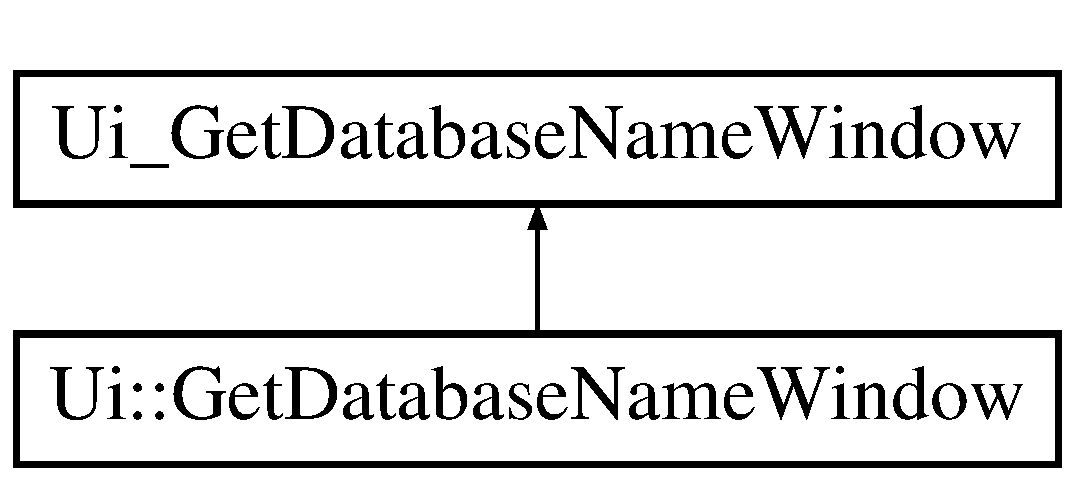
\includegraphics[height=2.000000cm]{class_ui___get_database_name_window}
\end{center}
\end{figure}
\subsection*{Public Member Functions}
\begin{DoxyCompactItemize}
\item 
\mbox{\Hypertarget{class_ui___get_database_name_window_abe670cb0626bd8c2db5f586b00297dd2}\label{class_ui___get_database_name_window_abe670cb0626bd8c2db5f586b00297dd2}} 
void {\bfseries setup\+Ui} (Q\+Dialog $\ast$\mbox{\hyperlink{class_get_database_name_window}{Get\+Database\+Name\+Window}})
\item 
\mbox{\Hypertarget{class_ui___get_database_name_window_ab7805601725849c954765cb3d0622f6d}\label{class_ui___get_database_name_window_ab7805601725849c954765cb3d0622f6d}} 
void {\bfseries retranslate\+Ui} (Q\+Dialog $\ast$\mbox{\hyperlink{class_get_database_name_window}{Get\+Database\+Name\+Window}})
\end{DoxyCompactItemize}
\subsection*{Public Attributes}
\begin{DoxyCompactItemize}
\item 
\mbox{\Hypertarget{class_ui___get_database_name_window_aa0b097e99fccc9a0d1dce24f4baf73a6}\label{class_ui___get_database_name_window_aa0b097e99fccc9a0d1dce24f4baf73a6}} 
Q\+Line\+Edit $\ast$ {\bfseries line\+Edit}
\item 
\mbox{\Hypertarget{class_ui___get_database_name_window_a8f9ded3034ed51d5ca0506c229e227a7}\label{class_ui___get_database_name_window_a8f9ded3034ed51d5ca0506c229e227a7}} 
Q\+Label $\ast$ {\bfseries title\+\_\+label}
\item 
\mbox{\Hypertarget{class_ui___get_database_name_window_a9a7bd6644ce7b668e0bb10349c48ee31}\label{class_ui___get_database_name_window_a9a7bd6644ce7b668e0bb10349c48ee31}} 
Q\+Label $\ast$ {\bfseries info\+\_\+label}
\item 
\mbox{\Hypertarget{class_ui___get_database_name_window_a061e2797af2bb551dbe0158c3d8f172f}\label{class_ui___get_database_name_window_a061e2797af2bb551dbe0158c3d8f172f}} 
Q\+Push\+Button $\ast$ {\bfseries add\+\_\+button}
\item 
\mbox{\Hypertarget{class_ui___get_database_name_window_a6f89ee4c6b8c056971a1c1e578f2d0e3}\label{class_ui___get_database_name_window_a6f89ee4c6b8c056971a1c1e578f2d0e3}} 
Q\+Push\+Button $\ast$ {\bfseries come\+\_\+back\+\_\+button}
\end{DoxyCompactItemize}


The documentation for this class was generated from the following file\+:\begin{DoxyCompactItemize}
\item 
ui\+\_\+getdatabasenamewindow.\+h\end{DoxyCompactItemize}

\hypertarget{class_ui___main_win}{}\section{Ui\+\_\+\+Main\+Win Class Reference}
\label{class_ui___main_win}\index{Ui\+\_\+\+Main\+Win@{Ui\+\_\+\+Main\+Win}}
Inheritance diagram for Ui\+\_\+\+Main\+Win\+:\begin{figure}[H]
\begin{center}
\leavevmode
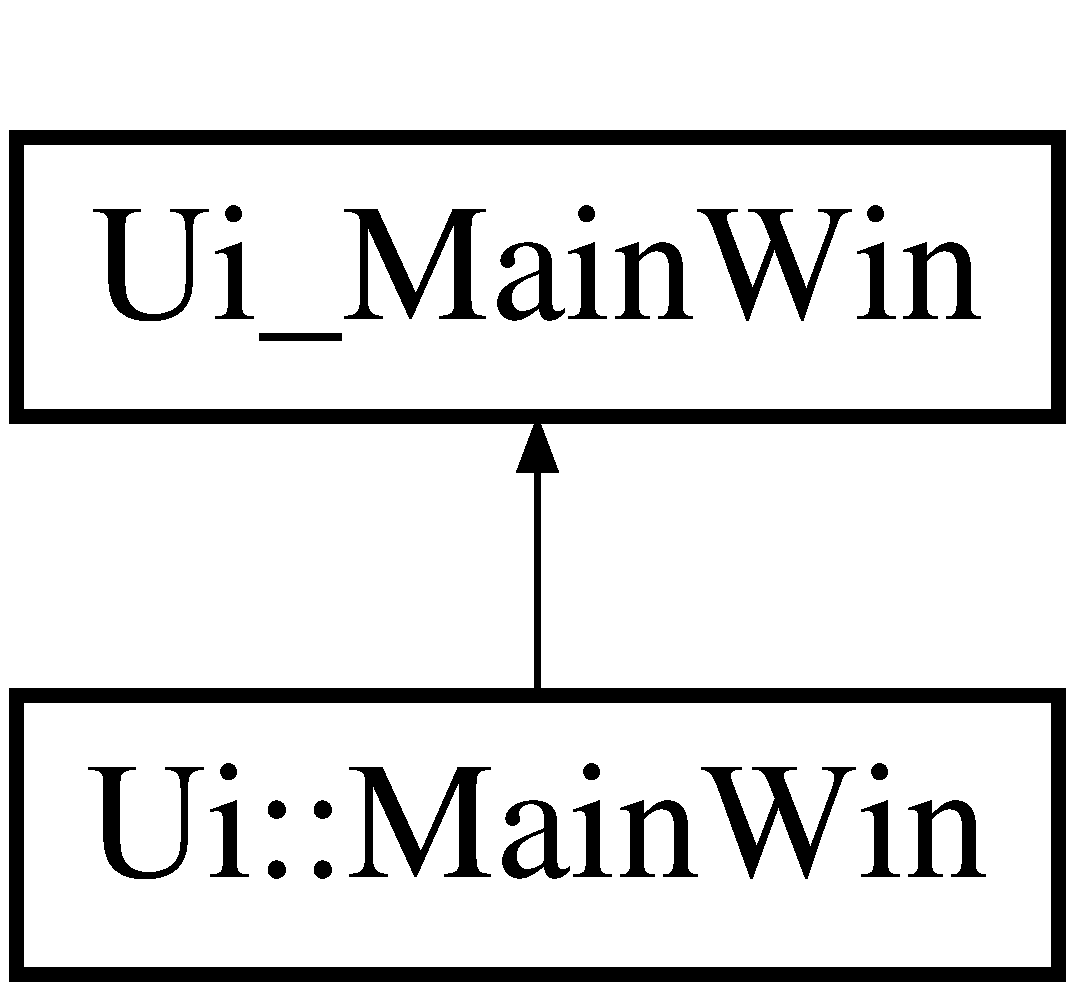
\includegraphics[height=2.000000cm]{class_ui___main_win}
\end{center}
\end{figure}
\subsection*{Public Member Functions}
\begin{DoxyCompactItemize}
\item 
\mbox{\Hypertarget{class_ui___main_win_a5d1d8e14b7878337a685fab66f26c28d}\label{class_ui___main_win_a5d1d8e14b7878337a685fab66f26c28d}} 
void {\bfseries setup\+Ui} (Q\+Main\+Window $\ast$\mbox{\hyperlink{class_main_win}{Main\+Win}})
\item 
\mbox{\Hypertarget{class_ui___main_win_a1bce8e2218d94fc5f3b2c90cf742886e}\label{class_ui___main_win_a1bce8e2218d94fc5f3b2c90cf742886e}} 
void {\bfseries retranslate\+Ui} (Q\+Main\+Window $\ast$\mbox{\hyperlink{class_main_win}{Main\+Win}})
\end{DoxyCompactItemize}
\subsection*{Public Attributes}
\begin{DoxyCompactItemize}
\item 
\mbox{\Hypertarget{class_ui___main_win_aa43c905850d7f50a5467788d14cf7fe0}\label{class_ui___main_win_aa43c905850d7f50a5467788d14cf7fe0}} 
Q\+Widget $\ast$ {\bfseries centralwidget}
\item 
\mbox{\Hypertarget{class_ui___main_win_adede7cfe504f4e4af09803d68eff5d16}\label{class_ui___main_win_adede7cfe504f4e4af09803d68eff5d16}} 
Q\+Widget $\ast$ {\bfseries horizontal\+Layout\+Widget}
\item 
\mbox{\Hypertarget{class_ui___main_win_a0d62a2b36cb344703803ef3438eba271}\label{class_ui___main_win_a0d62a2b36cb344703803ef3438eba271}} 
Q\+H\+Box\+Layout $\ast$ {\bfseries horizontal\+Layout}
\item 
\mbox{\Hypertarget{class_ui___main_win_a72e3b25031a3213358c48a1c996f434b}\label{class_ui___main_win_a72e3b25031a3213358c48a1c996f434b}} 
Q\+Label $\ast$ {\bfseries label\+\_\+2}
\item 
\mbox{\Hypertarget{class_ui___main_win_a9102e1c1bff7a71fe0d255c98c5fa728}\label{class_ui___main_win_a9102e1c1bff7a71fe0d255c98c5fa728}} 
Q\+Label $\ast$ {\bfseries label}
\item 
\mbox{\Hypertarget{class_ui___main_win_abd1ecf6b6dc733a0e1879cc75d991f03}\label{class_ui___main_win_abd1ecf6b6dc733a0e1879cc75d991f03}} 
Q\+Widget $\ast$ {\bfseries horizontal\+Layout\+Widget\+\_\+2}
\item 
\mbox{\Hypertarget{class_ui___main_win_ade0544e4541085a3d7c11ff04a5d08e9}\label{class_ui___main_win_ade0544e4541085a3d7c11ff04a5d08e9}} 
Q\+H\+Box\+Layout $\ast$ {\bfseries horizontal\+Layout\+\_\+2}
\item 
\mbox{\Hypertarget{class_ui___main_win_aaca3e18af100af24c4da1bbf106b2ec3}\label{class_ui___main_win_aaca3e18af100af24c4da1bbf106b2ec3}} 
Q\+Text\+Browser $\ast$ {\bfseries native\+\_\+word\+\_\+view}
\item 
\mbox{\Hypertarget{class_ui___main_win_a4af5b27964f7a1fc20dde05c0e7365c6}\label{class_ui___main_win_a4af5b27964f7a1fc20dde05c0e7365c6}} 
Q\+Text\+Browser $\ast$ {\bfseries foreign\+\_\+word\+\_\+view}
\item 
\mbox{\Hypertarget{class_ui___main_win_a901c9888ef08bfd60af50115c32162b7}\label{class_ui___main_win_a901c9888ef08bfd60af50115c32162b7}} 
Q\+Widget $\ast$ {\bfseries horizontal\+Layout\+Widget\+\_\+5}
\item 
\mbox{\Hypertarget{class_ui___main_win_a19ebcde7bcc6691b579c698fd814f3fb}\label{class_ui___main_win_a19ebcde7bcc6691b579c698fd814f3fb}} 
Q\+H\+Box\+Layout $\ast$ {\bfseries horizontal\+Layout\+\_\+5}
\item 
\mbox{\Hypertarget{class_ui___main_win_aa2c8358d98375295c8f56ced24847203}\label{class_ui___main_win_aa2c8358d98375295c8f56ced24847203}} 
Q\+Label $\ast$ {\bfseries label\+\_\+3}
\item 
\mbox{\Hypertarget{class_ui___main_win_ae7bef2876407ebff1d4347bc599355a7}\label{class_ui___main_win_ae7bef2876407ebff1d4347bc599355a7}} 
Q\+Text\+Browser $\ast$ {\bfseries descript\+\_\+view}
\item 
\mbox{\Hypertarget{class_ui___main_win_a6ebcef6787f8220daf8798b6e370af1c}\label{class_ui___main_win_a6ebcef6787f8220daf8798b6e370af1c}} 
Q\+Label $\ast$ {\bfseries image\+\_\+view}
\item 
\mbox{\Hypertarget{class_ui___main_win_a1730737dfeb3b54b3d653183f582137e}\label{class_ui___main_win_a1730737dfeb3b54b3d653183f582137e}} 
Q\+Push\+Button $\ast$ {\bfseries exit\+\_\+button}
\item 
\mbox{\Hypertarget{class_ui___main_win_a02d94095c3d351f63857a9ea83beaf20}\label{class_ui___main_win_a02d94095c3d351f63857a9ea83beaf20}} 
Q\+Push\+Button $\ast$ {\bfseries check\+\_\+button}
\item 
\mbox{\Hypertarget{class_ui___main_win_aaa22ec024c399b8c7a539789d72bf6ce}\label{class_ui___main_win_aaa22ec024c399b8c7a539789d72bf6ce}} 
Q\+Push\+Button $\ast$ {\bfseries dont\+\_\+know\+\_\+button}
\item 
\mbox{\Hypertarget{class_ui___main_win_a44eaafe353a42058df2fa5cf3a1faacc}\label{class_ui___main_win_a44eaafe353a42058df2fa5cf3a1faacc}} 
Q\+Push\+Button $\ast$ {\bfseries know\+\_\+button}
\item 
\mbox{\Hypertarget{class_ui___main_win_a68785e2d3a0379ad5dd01cc1192b18b0}\label{class_ui___main_win_a68785e2d3a0379ad5dd01cc1192b18b0}} 
Q\+Label $\ast$ {\bfseries image\+\_\+label}
\item 
\mbox{\Hypertarget{class_ui___main_win_a1177632545f78597de242758668f6152}\label{class_ui___main_win_a1177632545f78597de242758668f6152}} 
Q\+Status\+Bar $\ast$ {\bfseries statusbar}
\end{DoxyCompactItemize}


The documentation for this class was generated from the following file\+:\begin{DoxyCompactItemize}
\item 
ui\+\_\+mainwin.\+h\end{DoxyCompactItemize}

\hypertarget{class_ui___menu_start}{}\section{Ui\+\_\+\+Menu\+Start Class Reference}
\label{class_ui___menu_start}\index{Ui\+\_\+\+Menu\+Start@{Ui\+\_\+\+Menu\+Start}}
Inheritance diagram for Ui\+\_\+\+Menu\+Start\+:\begin{figure}[H]
\begin{center}
\leavevmode
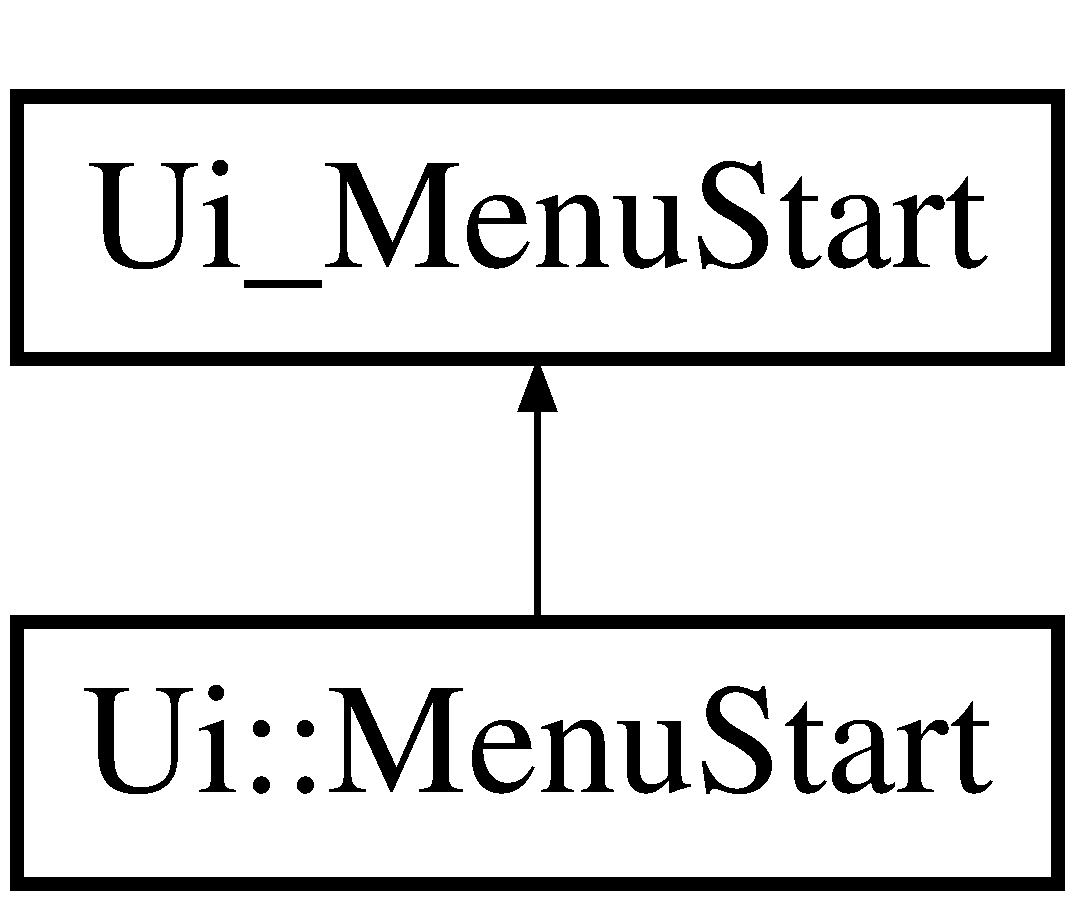
\includegraphics[height=2.000000cm]{class_ui___menu_start}
\end{center}
\end{figure}
\subsection*{Public Member Functions}
\begin{DoxyCompactItemize}
\item 
\mbox{\Hypertarget{class_ui___menu_start_a2c829c09e6c5cee3a6eb27777f41b4d7}\label{class_ui___menu_start_a2c829c09e6c5cee3a6eb27777f41b4d7}} 
void {\bfseries setup\+Ui} (Q\+Dialog $\ast$\mbox{\hyperlink{class_menu_start}{Menu\+Start}})
\item 
\mbox{\Hypertarget{class_ui___menu_start_aef0991221e943ae0621380cc743acec5}\label{class_ui___menu_start_aef0991221e943ae0621380cc743acec5}} 
void {\bfseries retranslate\+Ui} (Q\+Dialog $\ast$\mbox{\hyperlink{class_menu_start}{Menu\+Start}})
\end{DoxyCompactItemize}
\subsection*{Public Attributes}
\begin{DoxyCompactItemize}
\item 
\mbox{\Hypertarget{class_ui___menu_start_a77bad3a33dc6bfef2b26b75970666b0c}\label{class_ui___menu_start_a77bad3a33dc6bfef2b26b75970666b0c}} 
Q\+Widget $\ast$ {\bfseries grid\+Layout\+Widget}
\item 
\mbox{\Hypertarget{class_ui___menu_start_ab8cc6201812de4b859d4962848c60f04}\label{class_ui___menu_start_ab8cc6201812de4b859d4962848c60f04}} 
Q\+Grid\+Layout $\ast$ {\bfseries grid\+Layout}
\item 
\mbox{\Hypertarget{class_ui___menu_start_ac5bfb452ffedd7c21009ea5eb49a8fc5}\label{class_ui___menu_start_ac5bfb452ffedd7c21009ea5eb49a8fc5}} 
Q\+Push\+Button $\ast$ {\bfseries exit\+\_\+button\+\_\+}
\item 
\mbox{\Hypertarget{class_ui___menu_start_a951fba3ccfea001747e4e291ca7d32da}\label{class_ui___menu_start_a951fba3ccfea001747e4e291ca7d32da}} 
Q\+Push\+Button $\ast$ {\bfseries start\+\_\+learning\+\_\+button\+\_\+}
\item 
\mbox{\Hypertarget{class_ui___menu_start_a7c46ec686b19734be2ab86f66a95906a}\label{class_ui___menu_start_a7c46ec686b19734be2ab86f66a95906a}} 
Q\+Push\+Button $\ast$ {\bfseries delete\+\_\+database\+\_\+button\+\_\+}
\item 
\mbox{\Hypertarget{class_ui___menu_start_a32321cdffe5f4f100e3f0c5ddc83dd2f}\label{class_ui___menu_start_a32321cdffe5f4f100e3f0c5ddc83dd2f}} 
Q\+Push\+Button $\ast$ {\bfseries add\+\_\+database\+\_\+button\+\_\+}
\item 
\mbox{\Hypertarget{class_ui___menu_start_a9ee615f94113d4577eafdbb39cc4f0a2}\label{class_ui___menu_start_a9ee615f94113d4577eafdbb39cc4f0a2}} 
Q\+Label $\ast$ {\bfseries image\+\_\+label}
\end{DoxyCompactItemize}


The documentation for this class was generated from the following file\+:\begin{DoxyCompactItemize}
\item 
ui\+\_\+menustart.\+h\end{DoxyCompactItemize}

\hypertarget{class_word}{}\section{Word Class Reference}
\label{class_word}\index{Word@{Word}}


Klasa reprezentuje dane słówko, które może być zapisane w dwóch językach oraz posiadac pewien synonim lub opis. dostarcza funkcji umożliwających modyfikacje słówka oraz jego zapis i odczyt z /do pliku.  




{\ttfamily \#include $<$word.\+h$>$}

Inheritance diagram for Word\+:\begin{figure}[H]
\begin{center}
\leavevmode
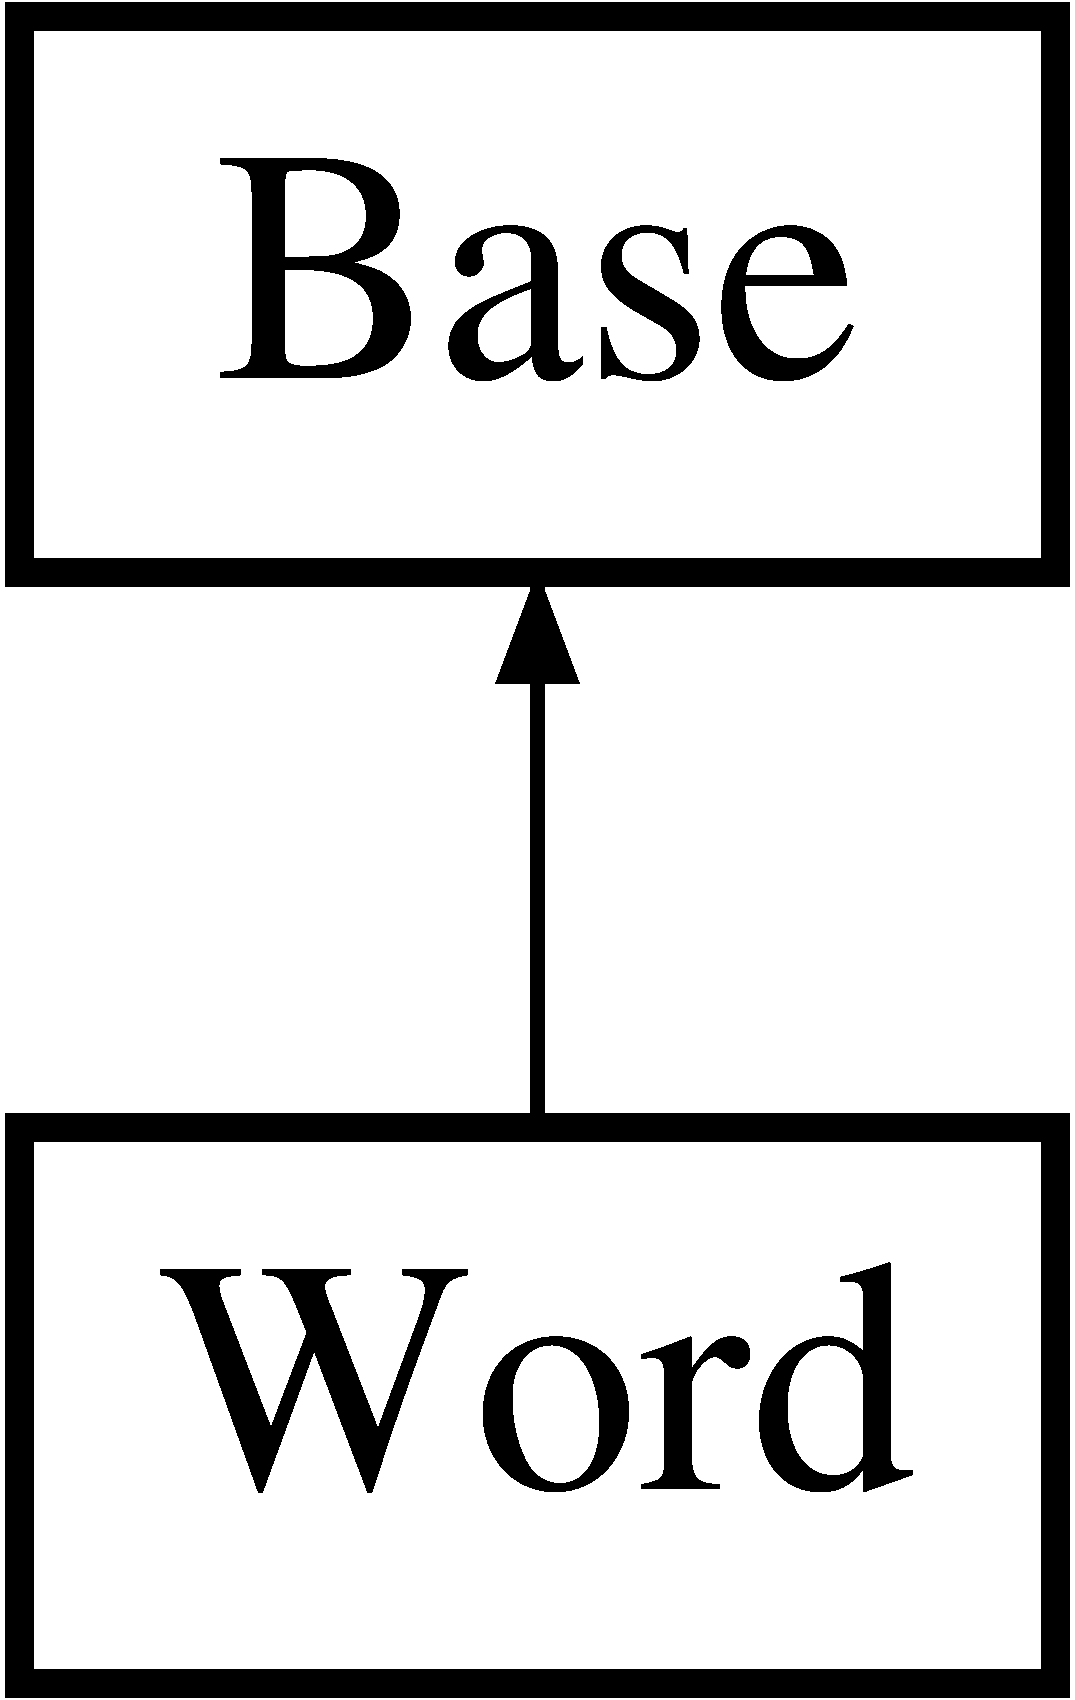
\includegraphics[height=2.000000cm]{class_word}
\end{center}
\end{figure}
\subsection*{Public Member Functions}
\begin{DoxyCompactItemize}
\item 
\mbox{\Hypertarget{class_word_aa7eab6629fdbc794f379ff7d1746979e}\label{class_word_aa7eab6629fdbc794f379ff7d1746979e}} 
{\bfseries Word} (std\+::string native, std\+::string foreign, std\+::string translate)
\item 
\mbox{\Hypertarget{class_word_a1e082803fada1b99cce469604fa5e4b4}\label{class_word_a1e082803fada1b99cce469604fa5e4b4}} 
virtual void {\bfseries import\+Data} (std\+::istream \&in\+\_\+)
\item 
\mbox{\Hypertarget{class_word_ae70c9ade266f84482e7bb1aeaafccb3b}\label{class_word_ae70c9ade266f84482e7bb1aeaafccb3b}} 
virtual void {\bfseries export\+Data} (std\+::ostream \&out\+\_\+)
\item 
\mbox{\Hypertarget{class_word_a89e6bd6b32eee3266752bdea037c7c2f}\label{class_word_a89e6bd6b32eee3266752bdea037c7c2f}} 
virtual std\+::string {\bfseries get\+Foreign\+Word} ()
\item 
\mbox{\Hypertarget{class_word_a8ec142e06e4a361a898bb13aef837e6d}\label{class_word_a8ec142e06e4a361a898bb13aef837e6d}} 
virtual void {\bfseries set\+Foreign\+Word} (std\+::string word)
\item 
\mbox{\Hypertarget{class_word_ad5b593288cc4b6db9e905751308a396b}\label{class_word_ad5b593288cc4b6db9e905751308a396b}} 
virtual std\+::string {\bfseries get\+Native\+Word} ()
\item 
\mbox{\Hypertarget{class_word_a35bf10ad12dbe48a30a6a8b2f96b2dc5}\label{class_word_a35bf10ad12dbe48a30a6a8b2f96b2dc5}} 
virtual void {\bfseries set\+Native\+Word} (std\+::string word)
\item 
\mbox{\Hypertarget{class_word_a167500076ba8a742ae6cad5dc1507361}\label{class_word_a167500076ba8a742ae6cad5dc1507361}} 
virtual std\+::string {\bfseries get\+Translation} ()
\item 
\mbox{\Hypertarget{class_word_ad583dd58318ebc7be4d5e02bcf173191}\label{class_word_ad583dd58318ebc7be4d5e02bcf173191}} 
virtual void {\bfseries set\+Translation} (std\+::string word)
\item 
\mbox{\Hypertarget{class_word_a182a4223aab6094d670166a8e3fdd8c0}\label{class_word_a182a4223aab6094d670166a8e3fdd8c0}} 
virtual void {\bfseries add} (\mbox{\hyperlink{class_base}{Base}} $\ast$)
\end{DoxyCompactItemize}
\subsection*{Additional Inherited Members}


\subsection{Detailed Description}
Klasa reprezentuje dane słówko, które może być zapisane w dwóch językach oraz posiadac pewien synonim lub opis. dostarcza funkcji umożliwających modyfikacje słówka oraz jego zapis i odczyt z /do pliku. 

The documentation for this class was generated from the following files\+:\begin{DoxyCompactItemize}
\item 
word.\+h\item 
word.\+cpp\end{DoxyCompactItemize}

%--- End generated contents ---

% Index
\backmatter
\newpage
\phantomsection
\clearemptydoublepage
\addcontentsline{toc}{chapter}{Index}
\printindex

\end{document}
